
%% bare_conf.tex
%% V1.3
%% 2007/01/11
%% by Michael Shell
%% See:
%% http://www.michaelshell.org/
%% for current contact information.
%%
%% This is a skeleton file demonstrating the use of IEEEtran.cls
%% (requires IEEEtran.cls version 1.7 or later) with an IEEE conference paper.
%%
%% Support sites:
%% http://www.michaelshell.org/tex/ieeetran/
%% http://www.ctan.org/tex-archive/macros/latex/contrib/IEEEtran/
%% and
%% http://www.ieee.org/

%%*************************************************************************
%% Legal Notice:
%% This code is offered as-is without any warranty either expressed or
%% implied; without even the implied warranty of MERCHANTABILITY or
%% FITNESS FOR A PARTICULAR PURPOSE! 
%% User assumes all risk.
%% In no event shall IEEE or any contributor to this code be liable for
%% any damages or losses, including, but not limited to, incidental,
%% consequential, or any other damages, resulting from the use or misuse
%% of any information contained here.
%%
%% All comments are the opinions of their respective authors and are not
%% necessarily endorsed by the IEEE.
%%
%% This work is distributed under the LaTeX Project Public License (LPPL)
%% ( http://www.latex-project.org/ ) version 1.3, and may be freely used,
%% distributed and modified. A copy of the LPPL, version 1.3, is included
%% in the base LaTeX documentation of all distributions of LaTeX released
%% 2003/12/01 or later.
%% Retain all contribution notices and credits.
%% ** Modified files should be clearly indicated as such, including  **
%% ** renaming them and changing author support contact information. **
%%
%% File list of work: IEEEtran.cls, IEEEtran_HOWTO.pdf, bare_adv.tex,
%%                    bare_conf.tex, bare_jrnl.tex, bare_jrnl_compsoc.tex
%%*************************************************************************

% *** Authors should verify (and, if needed, correct) their LaTeX system  ***
% *** with the testflow diagnostic prior to trusting their LaTeX platform ***
% *** with production work. IEEE's font choices can trigger bugs that do  ***
% *** not appear when using other class files.                            ***
% The testflow support page is at:
% http://www.michaelshell.org/tex/testflow/



% Note that the a4paper option is mainly intended so that authors in
% countries using A4 can easily print to A4 and see how their papers will
% look in print - the typesetting of the document will not typically be
% affected with changes in paper size (but the bottom and side margins will).
% Use the testflow package mentioned above to verify correct handling of
% both paper sizes by the user's LaTeX system.
%
% Also note that the "draftcls" or "draftclsnofoot", not "draft", option
% should be used if it is desired that the figures are to be displayed in
% draft mode.
%
\documentclass[10pt, conference, compsocconf]{IEEEtran}
% Add the compsocconf option for Computer Society conferences.
%
% If IEEEtran.cls has not been installed into the LaTeX system files,
% manually specify the path to it like:
% \documentclass[conference]{../sty/IEEEtran}





% Some very useful LaTeX packages include:
% (uncomment the ones you want to load)


% *** MISC UTILITY PACKAGES ***
%
%\usepackage{ifpdf}
% Heiko Oberdiek's ifpdf.sty is very useful if you need conditional
% compilation based on whether the output is pdf or dvi.
% usage:
% \ifpdf
%   % pdf code
% \else
%   % dvi code
% \fi
% The latest version of ifpdf.sty can be obtained from:
% http://www.ctan.org/tex-archive/macros/latex/contrib/oberdiek/
% Also, note that IEEEtran.cls V1.7 and later provides a builtin
% \ifCLASSINFOpdf conditional that works the same way.
% When switching from latex to pdflatex and vice-versa, the compiler may
% have to be run twice to clear warning/error messages.






% *** CITATION PACKAGES ***
%
%\usepackage{cite}
% cite.sty was written by Donald Arseneau
% V1.6 and later of IEEEtran pre-defines the format of the cite.sty package
% \cite{} output to follow that of IEEE. Loading the cite package will
% result in citation numbers being automatically sorted and properly
% "compressed/ranged". e.g., [1], [9], [2], [7], [5], [6] without using
% cite.sty will become [1], [2], [5]--[7], [9] using cite.sty. cite.sty's
% \cite will automatically add leading space, if needed. Use cite.sty's
% noadjust option (cite.sty V3.8 and later) if you want to turn this off.
% cite.sty is already installed on most LaTeX systems. Be sure and use
% version 4.0 (2003-05-27) and later if using hyperref.sty. cite.sty does
% not currently provide for hyperlinked citations.
% The latest version can be obtained at:
% http://www.ctan.org/tex-archive/macros/latex/contrib/cite/
% The documentation is contained in the cite.sty file itself.






% *** GRAPHICS RELATED PACKAGES ***
%
\ifCLASSINFOpdf
  % \usepackage[pdftex]{graphicx}
  % declare the path(s) where your graphic files are
  % \graphicspath{{../pdf/}{../jpeg/}}
  % and their extensions so you won't have to specify these with
  % every instance of \includegraphics
  % \DeclareGraphicsExtensions{.pdf,.jpeg,.png}
\else
  % or other class option (dvipsone, dvipdf, if not using dvips). graphicx
  % will default to the driver specified in the system graphics.cfg if no
  % driver is specified.
  % \usepackage[dvips]{graphicx}
  % declare the path(s) where your graphic files are
  % \graphicspath{{../eps/}}
  % and their extensions so you won't have to specify these with
  % every instance of \includegraphics
  % \DeclareGraphicsExtensions{.eps}
\fi
% graphicx was written by David Carlisle and Sebastian Rahtz. It is
% required if you want graphics, photos, etc. graphicx.sty is already
% installed on most LaTeX systems. The latest version and documentation can
% be obtained at: 
% http://www.ctan.org/tex-archive/macros/latex/required/graphics/
% Another good source of documentation is "Using Imported Graphics in
% LaTeX2e" by Keith Reckdahl which can be found as epslatex.ps or
% epslatex.pdf at: http://www.ctan.org/tex-archive/info/
%
% latex, and pdflatex in dvi mode, support graphics in encapsulated
% postscript (.eps) format. pdflatex in pdf mode supports graphics
% in .pdf, .jpeg, .png and .mps (metapost) formats. Users should ensure
% that all non-photo figures use a vector format (.eps, .pdf, .mps) and
% not a bitmapped formats (.jpeg, .png). IEEE frowns on bitmapped formats
% which can result in "jaggedy"/blurry rendering of lines and letters as
% well as large increases in file sizes.
%
% You can find documentation about the pdfTeX application at:
% http://www.tug.org/applications/pdftex





% *** MATH PACKAGES ***
%
%\usepackage[cmex10]{amsmath}
% A popular package from the American Mathematical Society that provides
% many useful and powerful commands for dealing with mathematics. If using
% it, be sure to load this package with the cmex10 option to ensure that
% only type 1 fonts will utilized at all point sizes. Without this option,
% it is possible that some math symbols, particularly those within
% footnotes, will be rendered in bitmap form which will result in a
% document that can not be IEEE Xplore compliant!
%
% Also, note that the amsmath package sets \interdisplaylinepenalty to 10000
% thus preventing page breaks from occurring within multiline equations. Use:
%\interdisplaylinepenalty=2500
% after loading amsmath to restore such page breaks as IEEEtran.cls normally
% does. amsmath.sty is already installed on most LaTeX systems. The latest
% version and documentation can be obtained at:
% http://www.ctan.org/tex-archive/macros/latex/required/amslatex/math/





% *** SPECIALIZED LIST PACKAGES ***
%
%\usepackage{algorithmic}
% algorithmic.sty was written by Peter Williams and Rogerio Brito.
% This package provides an algorithmic environment fo describing algorithms.
% You can use the algorithmic environment in-text or within a figure
% environment to provide for a floating algorithm. Do NOT use the algorithm
% floating environment provided by algorithm.sty (by the same authors) or
% algorithm2e.sty (by Christophe Fiorio) as IEEE does not use dedicated
% algorithm float types and packages that provide these will not provide
% correct IEEE style captions. The latest version and documentation of
% algorithmic.sty can be obtained at:
% http://www.ctan.org/tex-archive/macros/latex/contrib/algorithms/
% There is also a support site at:
% http://algorithms.berlios.de/index.html
% Also of interest may be the (relatively newer and more customizable)
% algorithmicx.sty package by Szasz Janos:
% http://www.ctan.org/tex-archive/macros/latex/contrib/algorithmicx/




% *** ALIGNMENT PACKAGES ***
%
%\usepackage{array}
% Frank Mittelbach's and David Carlisle's array.sty patches and improves
% the standard LaTeX2e array and tabular environments to provide better
% appearance and additional user controls. As the default LaTeX2e table
% generation code is lacking to the point of almost being broken with
% respect to the quality of the end results, all users are strongly
% advised to use an enhanced (at the very least that provided by array.sty)
% set of table tools. array.sty is already installed on most systems. The
% latest version and documentation can be obtained at:
% http://www.ctan.org/tex-archive/macros/latex/required/tools/


%\usepackage{mdwmath}
%\usepackage{mdwtab}
% Also highly recommended is Mark Wooding's extremely powerful MDW tools,
% especially mdwmath.sty and mdwtab.sty which are used to format equations
% and tables, respectively. The MDWtools set is already installed on most
% LaTeX systems. The lastest version and documentation is available at:
% http://www.ctan.org/tex-archive/macros/latex/contrib/mdwtools/


% IEEEtran contains the IEEEeqnarray family of commands that can be used to
% generate multiline equations as well as matrices, tables, etc., of high
% quality.

\usepackage[ruled,linesnumbered,lined]{algorithm2e}

%\usepackage{amsmath}
%\usepackage{enumitem}
%\usepackage{eqparbox}
% Also of notable interest is Scott Pakin's eqparbox package for creating
% (automatically sized) equal width boxes - aka "natural width parboxes".
% Available at:
% http://www.ctan.org/tex-archive/macros/latex/contrib/eqparbox/

\usepackage{graphicx}
\usepackage{subfigure}
\graphicspath{{figure/}}

\usepackage{hyperref}
\usepackage{multirow}
\usepackage{balance}
\usepackage{comment}
\usepackage{tikz}
\usepackage[numbers,sort&compress]{natbib}

\usepackage{color}
\definecolor{dkgreen}{rgb}{0,0.6,0}
\definecolor{gray}{rgb}{0.5,0.5,0.5}
\definecolor{mauve}{rgb}{0.58,0,0.82}
% Default settings for code listings

\newcommand{\tabincell}[2]{\begin{tabular}{@{}#1@{}}#2\end{tabular}}

\def\sharedaffiliation{
\end{tabular}
\begin{tabular}{c}}

% *** SUBFIGURE PACKAGES ***
%\usepackage[tight,footnotesize]{subfigure}
% subfigure.sty was written by Steven Douglas Cochran. This package makes it
% easy to put subfigures in your figures. e.g., "Figure 1a and 1b". For IEEE
% work, it is a good idea to load it with the tight package option to reduce
% the amount of white space around the subfigures. subfigure.sty is already
% installed on most LaTeX systems. The latest version and documentation can
% be obtained at:
% http://www.ctan.org/tex-archive/obsolete/macros/latex/contrib/subfigure/
% subfigure.sty has been superceeded by subfig.sty.

%\usepackage[caption=false]{caption}
%\usepackage[font=footnotesize]{subfig}
% subfig.sty, also written by Steven Douglas Cochran, is the modern
% replacement for subfigure.sty. However, subfig.sty requires and
% automatically loads Axel Sommerfeldt's caption.sty which will override
% IEEEtran.cls handling of captions and this will result in nonIEEE style
% figure/table captions. To prevent this problem, be sure and preload
% caption.sty with its "caption=false" package option. This is will preserve
% IEEEtran.cls handing of captions. Version 1.3 (2005/06/28) and later 
% (recommended due to many improvements over 1.2) of subfig.sty supports
% the caption=false option directly:
%\usepackage[caption=false,font=footnotesize]{subfig}
%
% The latest version and documentation can be obtained at:
% http://www.ctan.org/tex-archive/macros/latex/contrib/subfig/
% The latest version and documentation of caption.sty can be obtained at:
% http://www.ctan.org/tex-archive/macros/latex/contrib/caption/




% *** FLOAT PACKAGES ***
%
%\usepackage{fixltx2e}
% fixltx2e, the successor to the earlier fix2col.sty, was written by
% Frank Mittelbach and David Carlisle. This package corrects a few problems
% in the LaTeX2e kernel, the most notable of which is that in current
% LaTeX2e releases, the ordering of single and double column floats is not
% guaranteed to be preserved. Thus, an unpatched LaTeX2e can allow a
% single column figure to be placed prior to an earlier double column
% figure. The latest version and documentation can be found at:
% http://www.ctan.org/tex-archive/macros/latex/base/



%\usepackage{stfloats}
% stfloats.sty was written by Sigitas Tolusis. This package gives LaTeX2e
% the ability to do double column floats at the bottom of the page as well
% as the top. (e.g., "\begin{figure*}[!b]" is not normally possible in
% LaTeX2e). It also provides a command:
%\fnbelowfloat
% to enable the placement of footnotes below bottom floats (the standard
% LaTeX2e kernel puts them above bottom floats). This is an invasive package
% which rewrites many portions of the LaTeX2e float routines. It may not work
% with other packages that modify the LaTeX2e float routines. The latest
% version and documentation can be obtained at:
% http://www.ctan.org/tex-archive/macros/latex/contrib/sttools/
% Documentation is contained in the stfloats.sty comments as well as in the
% presfull.pdf file. Do not use the stfloats baselinefloat ability as IEEE
% does not allow \baselineskip to stretch. Authors submitting work to the
% IEEE should note that IEEE rarely uses double column equations and
% that authors should try to avoid such use. Do not be tempted to use the
% cuted.sty or midfloat.sty packages (also by Sigitas Tolusis) as IEEE does
% not format its papers in such ways.





% *** PDF, URL AND HYPERLINK PACKAGES ***
%
%\usepackage{url}
% url.sty was written by Donald Arseneau. It provides better support for
% handling and breaking URLs. url.sty is already installed on most LaTeX
% systems. The latest version can be obtained at:
% http://www.ctan.org/tex-archive/macros/latex/contrib/misc/
% Read the url.sty source comments for usage information. Basically,
% \url{my_url_here}.





% *** Do not adjust lengths that control margins, column widths, etc. ***
% *** Do not use packages that alter fonts (such as pslatex).         ***
% There should be no need to do such things with IEEEtran.cls V1.6 and later.
% (Unless specifically asked to do so by the journal or conference you plan
% to submit to, of course. )


% correct bad hyphenation here
\hyphenation{op-tical net-works semi-conduc-tor}


\begin{document}
%
% paper title
% can use linebreaks \\ within to get better formatting as desired
\title{MURS: Mitigating Memory Pressure in Data Processing Systems for Service}


% author names and affiliations
% use a multiple column layout for up to two different
% affiliations

\author{\IEEEauthorblockN{Xiong Zhang, Xuanhua Shi, Hai Jin, Song Wu, Zhixiang Ke}
\IEEEauthorblockA{Services Computing Technology and System Lab\\
Cluster and Grid Computing Lab\\
Big Data Technology and System Lab\\
School of Computer Science and Technology\\
Huazhong University of Science and Technology, Wuhan, 430074, China\\
Email: \{wxzhang, xhshi, hjin, wusong, zhxke\}@hust.edu.cn}
}

% conference papers do not typically use \thanks and this command
% is locked out in conference mode. If really needed, such as for
% the acknowledgment of grants, issue a \IEEEoverridecommandlockouts
% after \documentclass

% for over three affiliations, or if they all won't fit within the width
% of the page, use this alternative format:
% 
%\author{\IEEEauthorblockN{Michael Shell\IEEEauthorrefmark{1},
%Homer Simpson\IEEEauthorrefmark{2},
%James Kirk\IEEEauthorrefmark{3}, 
%Montgomery Scott\IEEEauthorrefmark{3} and
%Eldon Tyrell\IEEEauthorrefmark{4}}
%\IEEEauthorblockA{\IEEEauthorrefmark{1}School of Electrical and Computer Engineering\\
%Georgia Institute of Technology,
%Atlanta, Georgia 30332--0250\\ Email: see http://www.michaelshell.org/contact.html}
%\IEEEauthorblockA{\IEEEauthorrefmark{2}Twentieth Century Fox, Springfield, USA\\
%Email: homer@thesimpsons.com}
%\IEEEauthorblockA{\IEEEauthorrefmark{3}Starfleet Academy, San Francisco, California 96678-2391\\
%Telephone: (800) 555--1212, Fax: (888) 555--1212}
%\IEEEauthorblockA{\IEEEauthorrefmark{4}Tyrell Inc., 123 Replicant Street, Los Angeles, California 90210--4321}}




% use for special paper notices
%\IEEEspecialpapernotice{(Invited Paper)}




% make the title area
\maketitle


\begin{abstract}
In-memory computing systems are shown to suffer serious memory pressure as well as they are for service, the memory pressure will effect all submitted jobs. Memory pressure is coming from the running tasks as they produce massive long-lived data objects in limited memory, which brings significant memory and CPU overheads. Some tasks result in heavy memory pressure because of the operations and dataset they process, which affects all running tasks in the system. We find that each task includes several function APIs provided by the framework, and most function APIs produce long-lived data objects in memory within their own regular models; some need constant memory space while some need linear memory space. As different models have different impact on memory pressure, we propose memory usage rate to classify which model a task belongs to. Based on the memory usage rate, we design a scheduler called MURS to schedule all running tasks and mitigate heavy memory pressure. We implement MURS in Spark and the experimental study shows that, when compare to Spark, our scheduler can 1) decrease the execution time of submitted job by up to 58\%; 2) mitigate the memory pressure of all tasks by decreasing the garbage collection time by up to 94\%; and 3) avoid about 90\% of spill tasks to reduce disk I/O. 

\end{abstract}

\begin{IEEEkeywords}
memory pressure; memory usage rate; task scheduler; data processing systems for service

\end{IEEEkeywords}


% For peer review papers, you can put extra information on the cover
% page as needed:
% \ifCLASSOPTIONpeerreview
% \begin{center} \bfseries EDICS Category: 3-BBND \end{center}
% \fi
%
% For peerreview papers, this IEEEtran command inserts a page break and
% creates the second title. It will be ignored for other modes.
\IEEEpeerreviewmaketitle

\section{Introduction}

Many popular distributed data processing systems are sped up by in-memory computing model. Systems, such as Spark~\cite{zaharia2012resilient} and Flink~\cite{hueske2012opening}, are usually developed in Java, Scala and other managed languages. In-memory data are stored as data objects in memory, which can bloat the memory as shown in the literature~\cite{bu:bloat}. Limited memory space used by the submitted jobs will result in the memory pressure. Although these managed languages provide garbage collection(GC) to reclaim the useless data objects, caching data in memory may worsen the memory pressure as the data objects usually have a long lifetime in memory~\cite{lulu:deca}. 

Data processing systems usually work as batch processing systems. Jobs are submitted to systems individually and processed without the users' intervention. Many enterprises also deploy a data processing system as a server, such as Spark SQL~\cite{armbrust2015spark} and Hive~\cite{ashish:hive}. Multiple jobs are submitted to the system and executed in the same context. In addition to sharing the memory and CPU cores, the systems deployed as the services prefer caching the sharing data in memory in order to speed up all related jobs.
Some services are even oversold as they take the chance that all tenants may not submit their jobs at the same time. When these services process the tasks, multiple tasks are launched in the resources (such as a cluster), comparing with the original configurations where the tasks are processed by a service one by one. Data sharing and multiple launching both cause the heavy memory pressure, which in turn affects all jobs, although some jobs only cause the light memory pressure if they run alone in the batch processing mode.

%Many popular distributed systems are speed up by in-memory data in current days. These systems, such as Spark~\cite{zaharia2012resilient} and Flink~\cite{hueske2012opening}, are usually implemented by Java, Scala and other object-oriented languages. Caching data in memory is the most familiar measure for these frameworks. These caching data are stored in the JVM heap or off heap~\cite{www:tungsten} along with the runtime data objects in JVM heap. Besides the direct memory allocation for frameworks themselves, some resource managers ~\cite{vavilapalli2013apache}, distributed cache and distributed file systems~\cite{www:alluxio} also require memory to provide service for these frameworks ~\cite{pu2016fairride, li2014tachyon}. Based on the tense memory allocation, the memory pressure in frameworks themselves is already overwhelmed~\cite{fang2015interruptible}, especially when it provides service for multi tenant.

%There are two common ways, hot keys and large intermediate results, will lead to heavy memory pressure problem which harms the performance of data processing systems~\cite{fang2015interruptible}. Hot keys may result in an out-of-memory error, which may cause system crash. Large intermediate results, such as Java collection, may result in frequent garbage collection. The worst case occurs when the garbage collection time reaches a high percentage of execution time, performance of the data processing system will be extremely degraded, or system even crashes. In those systems for service, another particular problem is that some jobs have to suffer the inefficient memory pressure although they have light impact on memory. While most works mitigate memory pressure based on customized memory manager or application tuning in batch processing~\cite{www:spark-tuning, nguyen2015facade, fang2015interruptible, lulu:deca, nguyen:yak}, we intend to classify tasks those have greater impact on memory pressure in data processing systems for service. We briefly call task with greater impact on memory pressure as \textit{heavy task}, and task with light impact on memory pressure as \textit{light task}, respectively. Based on the classification, we suspend the heavy tasks to complete the light tasks, so that system resource is released and memory pressure is mitigated for all tasks.

Hot keys and large intermediate results are two common causes of the heavy memory pressure, which consequently harms the performance of data processing systems~\cite{fang2015interruptible}. Hot keys may result in an out-of-memory error, which may cause the system crash. Large intermediate results, such as Java collection, may lead to frequent garbage collection. When the garbage collection time becomes a big proportion of the entire execution time, the performance of the data processing system is significantly degraded. If the situation persists, the system may even crash. In the systems for service, another problem for the systems deployed as services is that some jobs have to suffer from the memory pressure although they cause light memory pressure themselves. Most works mitigate the memory pressure by customizing the memory managers or tuning the applications in batch processing~\cite{www:spark-tuning, nguyen2015facade, fang2015interruptible, lulu:deca, nguyen:yak}. In this work, we propose a new method to address this difficult issue. In the method, we classify the tasks in terms of memory pressure. A task that cause the heavy memory pressure is called a \textit{heavy task}, while the task with the light impact on memory called a \textit{light task}. Based on the classification, we suspend the heavy tasks so as to enable the light tasks to complete quickly. By doing so, the resources are released from running heavy tasks and the memory pressure is reduced for all tasks.

%Heavy memory pressure will break the performance of current data processing systems obviously in two common ways: hot keys and large intermediate results~\cite{fang2015interruptible}. Hot keys can result in out of memory error which can crash the system. About 40\% memory problems are related to large intermediate results, such as large Java collections. Large intermediate results can result in frequent garbage collection. The worst case is while the frequent garbage collection reclaims less space it results in the vicious circle and quickly declines the performance or even crashes systems. Systems for service cannot tolerant the heavy memory pressure much more because the heavy memory pressure may be resulted in by only parts of the running tasks. While most works mitigate the memory pressure based on the memory manger or long lived data objects in batch processing~\cite{fang2015interruptible, nguyen2015facade}, we intend to classify these tasks who have more impact on memory pressure in data processing systems for service. Based on the classification, tasks with less impact on memory pressure can break away from heavy memory pressure and release resource quickly to mitigate the memory pressure for other tasks.

%As memory pressure comes from massive long lived data objects produced by the running tasks in limited memory space, we find that the essential of long lived data objects is the function APIs called by tasks. These function APIs are based on key-value pairs~\cite{dean2008mapreduce, zaharia2012resilient, hueske2012opening, isard2007dryad} and the necessary memory space of different function APIs can be traced. The memory usage of these function APIs can be classified in four coarse-grained models: constant, sub-linear, linear, and super-linear. Each memory usage model has a different influence on memory. Task which is linear or super-linear model, or processing more input dataset, is closer to heavy task. These four models are combined independently in each task with strict order. We propose \textit{Memory Usage Rate} to determine to which model a task belongs. And we design a memory usage rate based scheduler, called MURS, which can efficiently mitigate heavy memory pressure and avoid memory overflow. The scheduler first collects the memory usage rate of current running tasks, and then selects the heavy tasks and suspend them. When heavy tasks are suspended, light tasks will complete quickly because memory pressure is light.

The memory pressure originates from massive long-living data objects produced by the running tasks in the limited memory space. Our studies further show that the root cause for generating these long-living data objects is the API functions called by the tasks. These function APIs are based on key-value pairs~\cite{dean2008mapreduce, zaharia2012resilient, hueske2012opening, isard2007dryad}. We find that the memory space used by the function APIs can be traced. The memory usage of the function APIs can be classified into four coarse-grained models: constant, sub-linear, linear and super-linear. Each memory usage model has a different influence on the memory pressure. The tasks with the linear or super-linear memory models, or the tasks that process more input dataset, are more likely to be the heavy tasks. These four models are combined independently in each task with a strict order. We propose the \textit{Memory Usage Rate} to determine which model a task belongs to. Further, we design a Memory-Usage-Rate based scheduler, called MURS, which can efficiently mitigate heavy memory pressure and avoid memory overflow. The scheduler first collects the memory usage rate of current running tasks, and then selects the heavy tasks and suspend them. After the heavy tasks are suspended, the light tasks can then complete quickly because of the light memory pressure. 

%As the memory pressure is coming from the massive long lived data object produced by the running tasks, tasks from different tenant will have different impact on memory pressure. Current data processing systems provide their own function APIs for user programs, and each task executes several function APIs~\cite{dean2008mapreduce, zaharia2012resilient, hueske2012opening, isard2007dryad}. We find that these function APIs are based on K-V pairs and the necessary memory space of different function APIs can be traced. The memory usage of these function APIs can be traced by four coarse-grained models: constant, sub-linear, linear and super-linear. Each model has different influence on memory, which means it can produce different memory pressure. Constant and sub-linear models have lighter effect on the memory pressure than linear model or super-linear model. These models are grouped independently in each task. We propose \textit{Memory Usage Rate} to distinguish which model one task belongs to. And we design a memory usage rate based scheduler called MURS which is proved to can avoid heavy memory pressure and spill. The scheduler gets the memory usage rate of current running tasks firstly, and chooses these tasks with linear or super-linear model to stop. When tasks with heavy influence on memory pressure is stopped, other tasks can complete quickly because memory pressure is light.

%Most works propose methods to slow down the memory pressure in batch processing, such as region based memory management~\cite{nguyen2015facade, gog2015broom}. However, the problem in multi-tenant is not always suited for these measures. Tenants who need less execution memory should not suffer heavy memory pressure poduced by other tenants. On the contrary, tenants who produce heavy memory pressure cannot get the resources of others immediately because others are prevented to complete early. The root of memory pressure is the running tasks who produce massive data objects in memory. Considering all tasks with the same characters is not appropriate in multi-tenant.

%Further more, users in both batch processing and multi-tenant write their codes by specific function APIs provided by frameworks, and then submit their jobs to system. As submitted job is always split into a set of tasks, each task executes several function APIs. Tasks running in the same time execute the same function APIs in batch processing but different function APIs in multi-tenant. Tasks with different function APIs have diverse effect on memory pressure undisputed, we find that although these tasks implement with the same function APIs, they can also have diverse effect on memory pressure because the distribution of keys in dataset also effect the memory pressure in some way. Thus, a uniform criterion to mark the influence on memory pressure of different tasks is most helpful to mange the tasks for both batch processing and multi-tenant.

%// 重点改



%In this paper, we analyze the characters of common function APIs in current popular data processing systems firstly. We propose \textit{Memory Usage Rate} to measure the influence one task has on the memory pressure. Four coarse grained types are designed to stand for different characters: constant, sub-linear, linear and super-linear. Constant tasks and sub-linear tasks have lighter effect on the memory pressure than linear tasks or super-leaner tasks. Based on the memory usage rate of current running tasks, we design a scheduler called MURS to schedule the tasks and avoid heavy memory pressure. The scheduler gets the memory usage rate of current running tasks in time and proposes the super linear or linear tasks to stop when the memory pressure comes. These stopped tasks will prevent heavy memory pressure because the heavy memory pressure is resulted in by themselves. Other tasks can run more quickly to empty the memory space for the stopped tasks.

%Last but not the least, we provide multi-launch to efficiently use memory. When light tasks have a large proportion in the running tasks, memory pressure is not heavy. Multi-launch will launch more tasks than original configuration to increase the parallelism as well as the memory pressure. In MURS, high parallelism can speed up the execution without considering heavy memory pressure. The multi-launch can be shut down optionally when the CPU resource is limited.

%Last but not the least, stopping tasks of some jobs is not appropriate in some way. Thus we provide multi launch to balance the stop, which can 1) speed up the occur of memory pressure and the response time for all submitted jobs; 2) increase the memory usage when all tasks have light pressure on memory by increasing parallelism. High parallelism instead of more memory pressure can improve the performance in some way. 

We implement MURS in Spark and conduct the extensive experiments. The experiments results shows that the execution time can be reduced by up to 65.8\% (2.9X). The garbage collection, which directly measures the memory pressure, can decrease by a maximum of 81\%. MURS can also help improve the scalability of the system, as the system equipped with MURS can still provide high quality of service even if the memory is in shortage. 

In summary, this work offers the following three main contributions.

\begin{itemize}

\item We analyze the memory utilization of various data processing systems, and find that the memory pressure originates from the function APIs called by the data processing frameworks when running the tasks. The invocation of the API functions generate massive long living data objects, which consume a large amount of memory.
%\item We propose memory usage rate which is bound to each task as a unified criterion for distinguishing their memory usage models in data processing systems for service. The criterion can extend to most data processing systems.

\item Based on our findings, we build four memory usage models to measure the impact a task has on memory pressure. The proposed models are independent of the data processing systems (and their function APIs). We also propose to use memory usage rate to identify which model a task belongs to. We design the memory usage rate based scheduler called MURS, which releases the memory pressure substantially.

%\item We propose multi launch to speed up the advent of memory pressure and increase the parallelism. The balance of pressure and parallelism can also improve the performance in some sense.

\item We implement a prototype system of MURS based on Spark. The proposed method can be ported to other similar data processing systems. The experimental results have shown that our system can significantly improve system performance, reduce garbage collection and extend the scalability of server.

\end{itemize}

The rest of the paper is organized as follows. Section II introduces the motivation of our work. Section III describes the four types of memory usage rate. Section IV characterizes the scheduler with the tasks with different memory usage rates. Section V presents the implementation of MURS; Performance evaluation is carried out in Section VI to show the advantages of our scheduler. In Section VII, we discuss the related work. Finally, Section VIII concludes the paper.
\section{Motivation}
\label{sec:motivation}

Memory is a critical type of resource in current data processing systems, especially in the in-memory computing systems~\cite{shi:mammoth}. Limited memory space leads to memory pressure and can cause frequent garbage collection or out-of-memory errors~\cite{fang2015interruptible}, both of which seriously affect the performance of the data processing system. A data processing system is often deployed as a batch processing system, but can also be deployed as a service and work as a service-oriented system. To understand the impact of memory pressure on the data processing systems and identify the cause of inefficiency, we investigate the running of the tasks with different memory requirements. We choose two types of applications, PageRank(PR) and WordCount(WC), which are the common benchmarks in Spark. The input dataset of PR and WC are webbase-2001 (30GB) and HiBench Random Writer (50GB). Spark can also work as a service-oriented system through the Spark Job Server. We first run the tasks in the service-oriented mode, in which we submit PR and WC simultaneously to the service-oriented Spark and run them with a fair scheduler in Spark. As a comparison, we also run PR and WC in the batch mode, in which PR and WC are processed one after the other. We record the execution times and garbage collection times of all tasks under these two modes, which are plotted in Figure~\ref{fig:memorypressure}. We then analyze the  memory pressure through the results.   

\begin{figure}[!t]
\centering
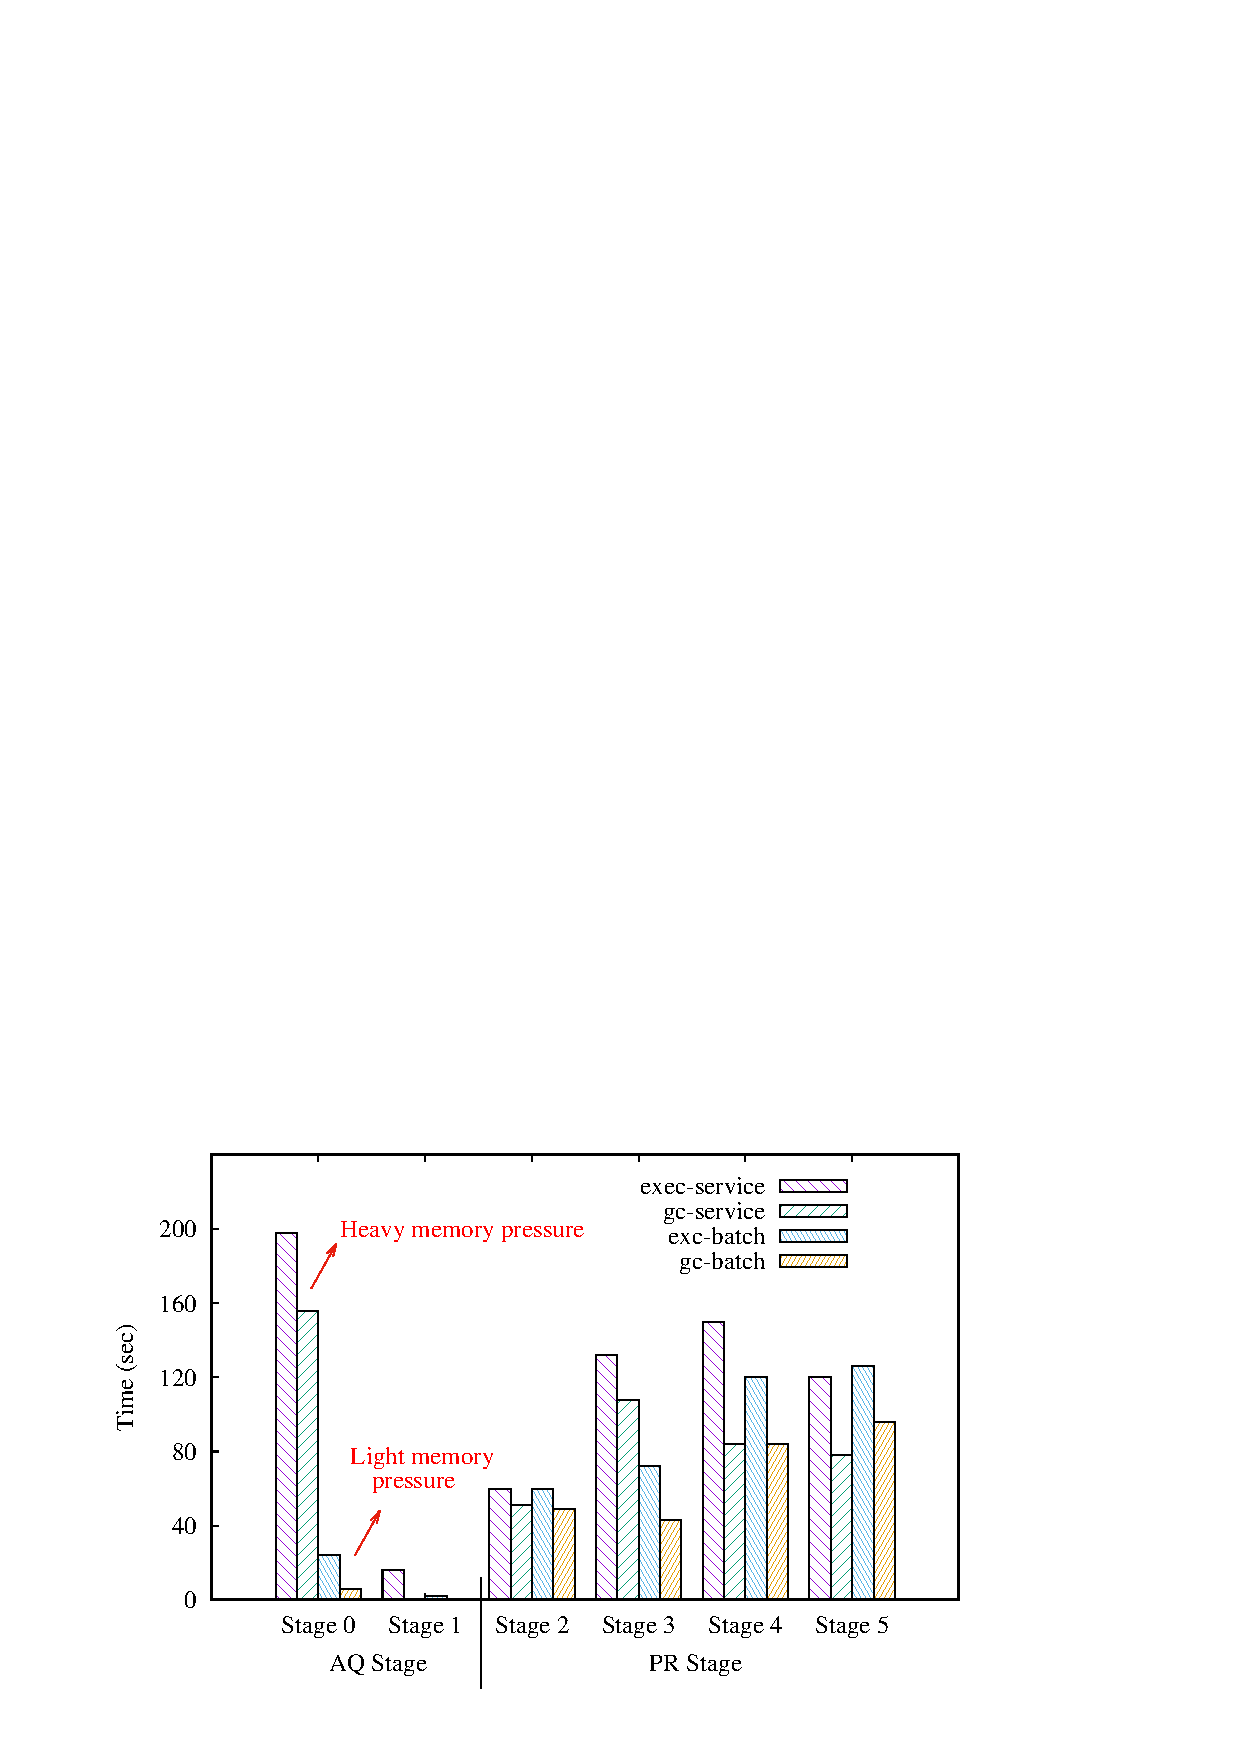
\includegraphics[width=0.35\textwidth]{motivation-exec-gc.pdf}
\vspace{-2mm}
\caption{WC suffers memory pressure from PR}
\vspace{-6mm}
\label{fig:memorypressure}
\end{figure}

We observe that PR caches intermediate data in memory and iteratively compute the result. One iteration corresponds to one stage in Spark. Because the caching data is alive as long as the job itself, the memory space becomes gradually less and the task computation will suffer. 
%If this occurs, it indicates the memory pressure caused by PR is heavy. 
Compare with PR, however, WC only contains some simple operations. WC has only two processing stages and during its execution, a very small amount of intermediate shuffle data are generated (although the input data of WC is larger than that of PR). 
%Furthermore, both the execution time and garbage collection time are low in WC, and the memory pressure is much lighter than PR. The result of PR in the batch mode also verifies its high memory pressure and heavy garbage collection, which are the results labelled as exec-batch and gc-batch in Figure~\ref{fig:memorypressure}. As we can see, the garbage collection time accounts for a very large proportion of the execution time.

When multiple jobs, such as PR and WC, are submitted to and run by the Spark service simultaneously, the jobs are run with a fair scheduler provided by Spark. Although WC has much more light memory pressure than PR, all running tasks suffer from the heavy memory pressure produced by PR. We find that the execution time (exec-service in Figure~\ref{fig:memorypressure} of every task in each stage of PR has little change
%, except some maximum execution times. This is because almost all memory pressure comes from PR and therefore the executions of PR in the service mode and the batch mode show similar trends
. However, The execution of WC in the service mode is very different from that in the batch mode. This is because in the service mode, both applications are run simultaneously and therefore WC suffers from the memory pressure produced by PR even if WC is a light task itself. 
%In the batch mode, since the applications are run one after another. The high memory pressure created by PR will not affect the running of WC.

In summary, our results implicate that in a service-oriented system, 1) the heavy memory pressure will result in frequent garbage collection, which consumes most of the time and reduces the throughput; 2) the light tasks suffer from heavy memory pressure produced by the heavy tasks; and 3) the heavy tasks obtain the resources later because these resources are occupied chronically by light tasks.
%, and the heavy tasks themselves are the source of memory pressure.

By observing the first stage of PR and WC, we discover that the tasks of PR and WC invoke different function APIs, which determine the impact of each task on memory pressure. If we can identify and classify these tasks by the characteristics of the function APIs, we can suspend the heavy tasks and leave adequate memory space to the light tasks when the memory pressure shows up. This can improve the throughput of the service-oriented systems and allow all tasks to run with enough memory space and hence light memory pressure. 
  

\section{Memory Usage Model in Tasks}

%// 模型的作用是什么没有说

%// 1,这些丰富的function API的特征是什么
%// 2,分类的原因
%// 3,通过实验证明有这四类的分类

As discussed in previous section, some tasks consume less memory while some use much more memory as they produce massive long living data object, which are mainly generated by function APIs in the processing pipeline. Although there are various function APIs, some of them manifest a similar characteristic in terms of memory usage. Based on this observation, we build the models to capture the memory usage characteristic of a function API, and then the memory usage rate is used to determine which model the task belongs to.

%We find that we can build models to describe the memory usage characteristics of a task. Tasks in some models can produce less memory pressure than others because they use less memory to complete the work. One of the major reason is the function APIs in the processing pipeline. Although different frameworks provide different function APIs, they all have similar characteristics when measuring memory usage. We can use memory usage rate to determine to which model the function APIs belong.

\subsection{Memory usage models of APIs}

\begin{comment}
\begin{table*}[!t]
\small
\centering
\caption{Function APIs in Distributed Data Processing System} 
\begin{tabular}{ c | c | c | c | c | c | c }

\hline
\multirow{2}{*}{\textbf{Community}} & \multicolumn{2}{|c|}{ \multirow{2}{*}{\textbf{Core API} }} & \multirow{2}{*}{\textbf{Application Systems}} & \multicolumn{3}{|c}{\textbf{Partial Function APIs}} \\
\cline{5-7}
 & \multicolumn{2}{|c|}{} & & constant & sub-linear & linear \\
\hline
Hadoop & MapRedcue~\cite{vavilapalli2013apache} & Crunch & Pig, Hive, Yarn & map & reduce & \\
\hline
Microsoft & Drayd~\cite{isard2007dryad} & DryadLINQ & Scope, MadLINQ & map & reduce & join \\
\hline
Spark & \multicolumn{2}{|c|}{RDD~\cite{zaharia2012resilient}} & Spark SQL~\cite{armbrust2015spark}, GraphX~\cite{xin2013graphx} & map & reduceByKey & groupByKey \\
\hline
Flink & \multicolumn{2}{|c|}{Dataset~\cite{www:flink}} & Table~\cite{www:flink}, Gelly~\cite{www:gelly} & where & distinct & join \\
\hline
Google & MapReduce & FlumeJava~\cite{flumejava} & Tenzing, Pregel, Sibyl & parallelDo & combinValue & groupByKey \\
\hline

\hline
\end{tabular}
\vspace{-2mm}
%\vspace{-4mm}
\label{table:apps}
\end{table*}
\end{comment}

A data processing system provides several function APIs, which can be used to implement various applications. 
%These function APIs take as input the input dataset and produce another dataset. The type of data in the dataset may be different. Table~\ref{table:apps} lists the function APIs provided by popular data processing systems. Most function APIs are sourced from MapReduce, a famous computing framework. Other function APIs are used to control the execution of jobs, the typical case of which is the shuffle operations. The shuffle operations are used between the \textit{Map} and the \textit{Reduce} phase, and are regarded as the separation point of a job, because the tasks after the shuffle operations (i.e., \textit{Reduce} tasks) need all results calculated by the tasks before the shuffle operations (\textit{Map} tasks).
These function APIs are all based on key-value pairs: (\textit{K}, \textit{V}). Some function APIs omit the parameter \textit{K} or \textit{V} for the convenience of users.
% Rather, the default value of the omitted parameters are used during the processes of \textit{map} or \textit{reduce}. The memory space is used by a function API to store the living data objects, because temporary data objects will be reclaimed by the garbage collection. 
The memory demand determines the characteristic of memory usage. Based on the key-value pairs, the memory size of living data objects is related to both \textit{K} and \textit{V} in the following ways.

\begin{itemize}

\item If the function API does not distinguish the parameter \textit{K}, it processes a record without involving other records. A record will produce a new record accordingly. If the new record is cached in memory, the consumed memory size will certainly increase. If the new record is processed as the input of the next function API or write-to-disk, it will be regarded as a temporary data object and quickly transmitted to the next function API. The size of temporary data object is ignored as it will be reclaimed in the next round of garbage collection.

\item If the function API distinguishes \textit{K}, it will involve all records to process these records with a particular \textit{K}. The function APIs that involve all records are usually called shuffle. While the shuffling stage processes the records to get all \textit{V} with a particular \textit{K}, two operations can be performed on \textit{V}: aggregation and non-aggregation.

\item If the function API does not aggregate the \textit{V}, it only puts \textit{V} in a collection without involving other \textit{V}. The collection contains the intermediate data and has a long lifetime because it is alive until the task processes all records. The collection is usually called the shuffle buffer. After a record is processed, the size of the collection increases by one element and thus the memory size of the shuffle buffer must increase.

\item If the function API aggregates the \textit{V}, the intermediate collection will be replaced by the aggregated value. We also call these data objects with long lifetime the shuffle buffer. Aggregation of \textit{V} means some operations will be performed on all \textit{V} with a particular \textit{K} and produce a new value. Thus, the resulting memory size of the collection will increase when \textit{K} has not appeared yet.

\end{itemize}

As the operations on \textit{K} and \textit{V} decide the size of the living data objects in memory, we build four models in this work to measure the memory usage of each function API when it processes a unit of data. 
%The models are based on the size of the records that are processed, not on the number of the processed records, because the size of a record in each dataset is different. 
Memory usage refers to the memory space used to store the data objects with long lifetime except the garbage data objects. The four models are shown in Figure~\ref{fig:mur}. 
%We determine the memory usage model of a function API by using the following lemmas.

If 1) the function API does not distinguish the key and 2)
the result data will not be cached in memory, then the memory
usage model of this function can be defined as \textit{constant} (Line
I in Figure~\ref{fig:mur}). If 1) the function API distinguishes the key and aggregates the values and 2) the key appears randomly in the
input dataset, then the memory usage model of this function can
be defined as \textit{sub-linear} (Line II in Figure~\ref{fig:mur}). Note that the
reason why we require that \textit{K} appears randomly is because
the size of intermediate data will increase only when the \textit{K}
has appeared. If most \textit{K}s gather around the neighbouring
records, the size of intermediate data will increase linearly.
Finally, if 1) the function API distinguishes \textit{K} but 2) it does not
aggregate \textit{V}, the memory usage model can be defined as
\textit{linear} (Line III in Figure~\ref{fig:mur}) (see~\cite{full} for details).

\begin{comment}
\begin{figure}[!t]
\centering
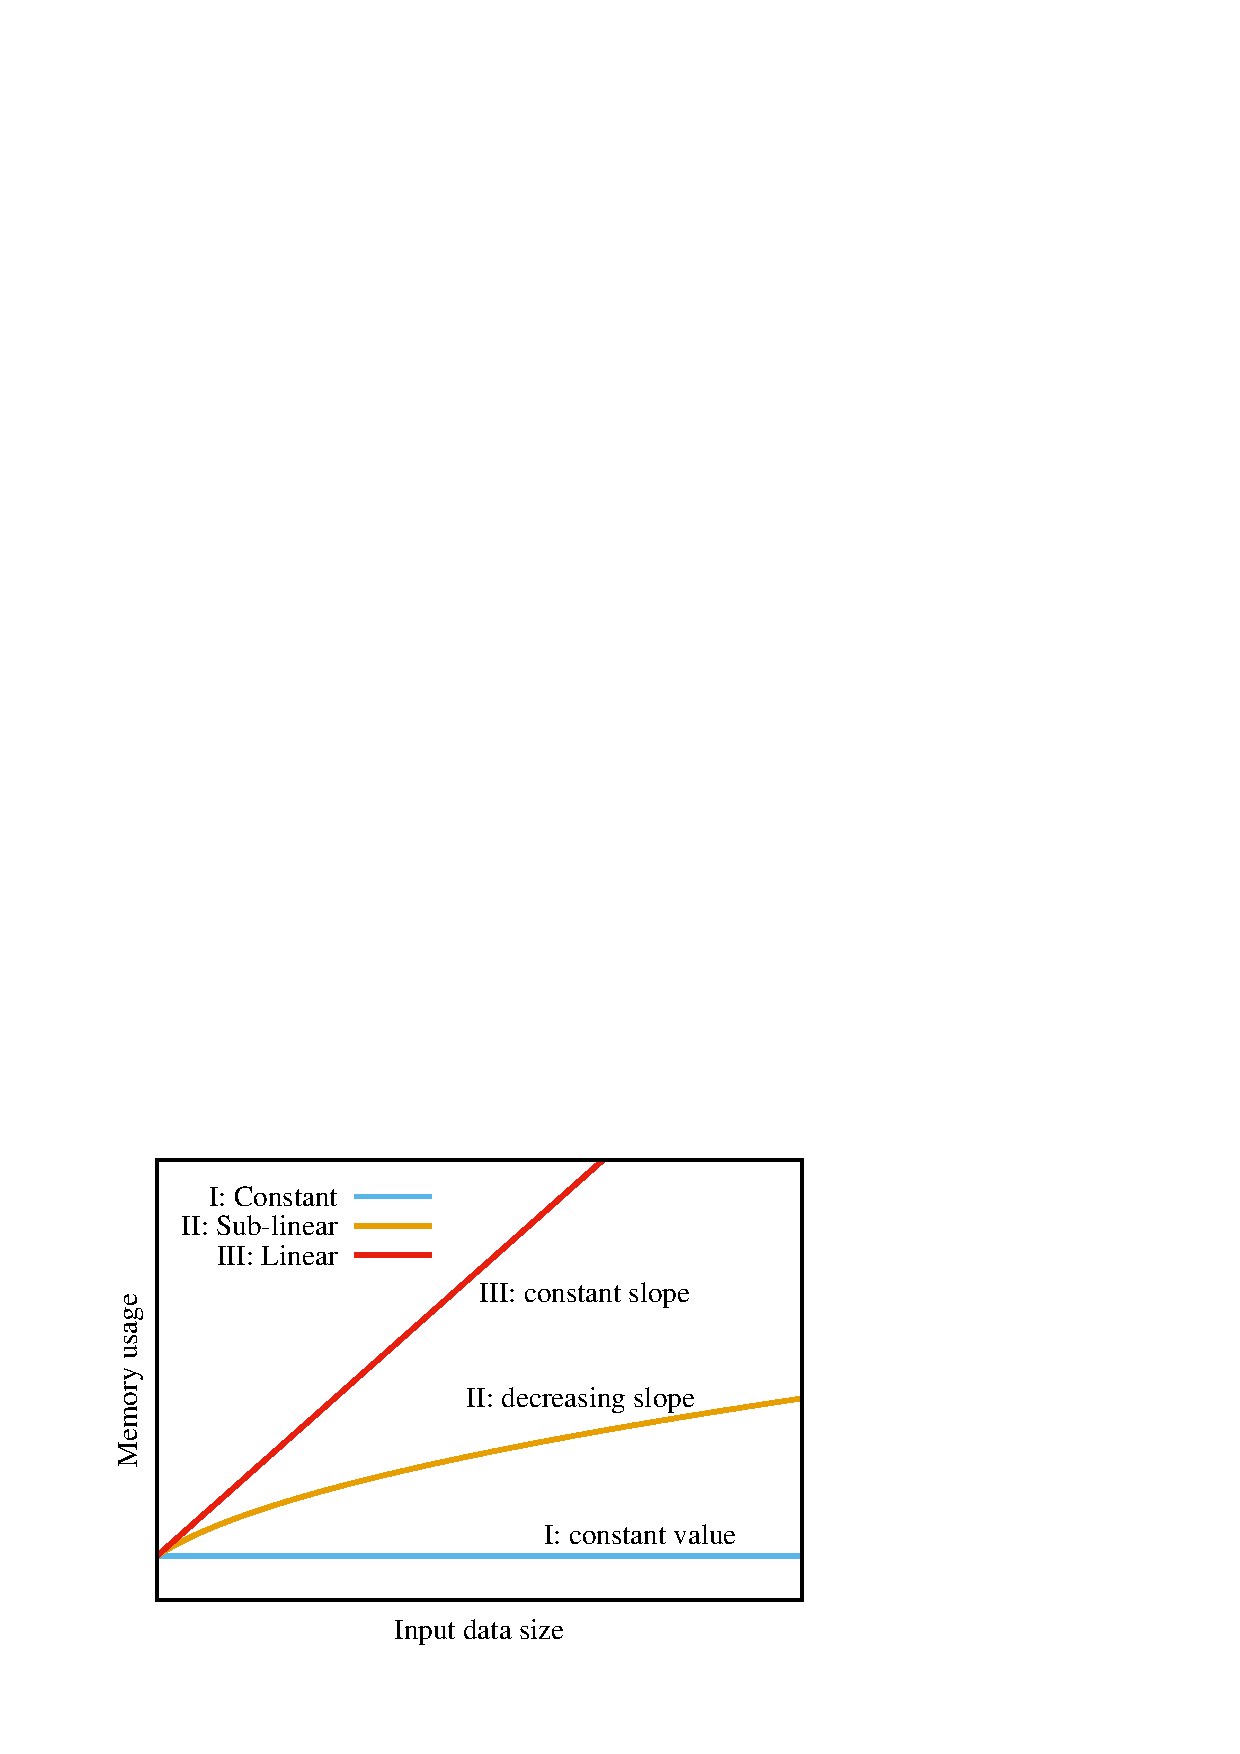
\includegraphics[width=0.3\textwidth]{mur.pdf}
\vspace{-2mm}
\caption{Four coarse-grained models of function API}
\vspace{-4mm}
\label{fig:mur}
\end{figure}

\newtheorem{lemma}{Lemma}
\begin{lemma}[Constant] The memory usage model can be defined as constant (Line I in Figure~\ref{fig:mur}) only when the following conditions are true:
\begin{enumerate}
\item The function API does not distinguish the key, \textit{K};
\item The resulting data will not be cached in memory.
\end{enumerate}
\end{lemma}

\begin{lemma}[Sub-Linear] The memory usage model can be defined as sub-linear (Line II in Figure~\ref{fig:mur}) only when the following conditions are true:
\begin{enumerate}
\item The function API distinguishes the key, \textit{K};
\item The function API aggregates the value, \textit{V};
\item \textit{K} appears randomly in the input dataset.
\end{enumerate}
\end{lemma}

Note that the reason why we require that \textit{K} appears randomly is because the size of intermediate data will increase only when the \textit{K} has appeared. If most \textit{K} gathers around some neighbouring records, the size of intermediate data will increase linearly.

\begin{lemma}[Linear] The memory usage model can be defined as linear (Line III in Figure~\ref{fig:mur}) when the following conditions hold:
\begin{enumerate}
\item The function API distinguishes \textit{K};
\item The function API does not aggregate \textit{V}.
\end{enumerate}
\end{lemma}
\end{comment}

Both cache operations and the appearance pattern of \textit{K} affect the  size of intermediate data. 
%Thus although some function APIs have the same operations on \textit{K} and \textit{V}, their memory usage models may be different. The constant model requires that intermediate data are not cached in memory. The increasing model is determined by the size of the cached data objects. The sub-linear model also requires the random appearance of \textit{K}. When a function API does not satisfy the above conditions, we need to redefine their models. In other words, the model is defined not only by the function APIs, but also by the user-defined function or data distribution. 
The memory usage model should be redefined when the following conditions are true.
If the function API does not distinguish the \textit{K} and the result data are cached in memory, the speed of increasing size in memory can be 1) \textit{linear} (Line III in Figure~\ref{fig:mur}) when the function API does not work based on formal result; 2) \textit{super-linear} (Line IV in Figure~\ref{fig:mur}) when the function API produces larger result data, such as computing a histogram of the appeared numbers and all their divisors; 3) \textit{sub-linear} (Line II in Figure~\ref{fig:mur}) when the function API produces smaller result data along with the computation.
If a function API i) distinguishes \textit{K}, ii) does not aggregate \textit{V}, iii) \textit{K} has not appeared yet in the input dataset or the appearance of \textit{K} is not random. The memory usage model of the function API should be linear.

\begin{comment}
\begin{itemize}

\item If the function API does not distinguish the \textit{K} and the result data are cached in memory, the speed of increasing size in memory can be 1) \textit{linear} (Line III in Figure~\ref{fig:mur}) when the function API does not work based on formal result; 2) \textit{super-linear} (Line IV in Figure~\ref{fig:mur}) when the function API produces larger result data, such as computing a histogram of the appeared numbers and all their divisors; 3) \textit{sub-linear} (Line II in Figure~\ref{fig:mur}) when the function API produces smaller result data along with the computation. 

\item If a function API i) distinguishes \textit{K}, ii) does not aggregate \textit{V}, iii) \textit{K} has not appeared yet in the input dataset or the appearance of \textit{K} is not random. The memory usage model of the function API should be linear.

\end{itemize}
\end{comment}

%Note that when function APIs belong to the same linear model, they can also be distinguished because the slope of the line in Figure~\ref{fig:mur} may be different. Steeper the slope is, the heavier impact the API function has on memory pressure. Based on the slope and four models, we can distinguish all function APIs in various data processing systems.

%If one function API does not satisfy one of the lemmas, we define them as the super-linear model. One possible super-linear model is shown as the Line IV in the figure. However, we find that no function API can be defined as the super-linear within the range of our research, most function APIs will show the memory usage as other three models in our evaluations.

%We should notice that the caching data and shuffle buffers are both long lifetime data objects in memory. Shuffle buffers are lived along with the shuffle operation. Some systems provide combine in map side which will effect the shuffle operation. When tasks need combine in map side, the function API will be executed in both map tasks (write) and reduce tasks (read). But when it needs not to combine, the function API will only be executed in reduce tasks, the map tasks will just produce the K-V pairs without any process. Other temporary data objects in function APIs will be reclaimed by garbage collection immediately.

%Some function APIs need both ensured \textit{K} and \textit{V}, such as \textit{shuffle}. According to the operations implemented on the \textit{V} with the same \textit{K}, these shuffle function APIs can be split to two groups: aggregate and non-aggregate. Aggregate operations are used to aggregate \textit{V} with the same \textit{K}. In this case, whether the result data in memory should increase the size is decided by the \textit{K}. But it's sure that non-aggregate operations must increase the size of result data in memory because no matter whether the \textit{K} has repeated emergence, \textit{V} is appended to the result data. What's more, besides the operations themselves affect the memory pressure, the type of \textit{V} also make some impact on the memory pressure. While the operations in running tasks are the same, we can also distinguish the influence on memory pressure by the data class they process.

%Some frameworks directly provide the \textit{cache} function API to cache the data in memory. This operation is different to other operations because it just applies for a memory space to store the dataset. JVM heap is usually the default region to store these data. Forward frameworks also provide storing off heap to save the execution memory space. No matter where the dataset store in, we just regard these memory pressure from JVM heap or system memory as unify.

%Most function APIs can satisfy these three items. Other function APIs, such as \textit{cache}, are designed to lengthen the lifetime of intermediate data but not influence the memory usage during processing. Further function APIs are also used to control the execution of jobs, the typical case is shuffle operations. Shuffle operations are used between Map and Reduce, and regarded as the break point of jobs. Because tasks after shuffle operations (reduce tasks) need all results of tasks before shuffle operations (Map tasks).  

\subsection{Memory usage models in tasks}
\label{subsec:taskmodel}

%A task is implemented by at least one function API. 
Some systems define only one function API in each task, such as Hadoop. Other systems define the function APIs in a task according to the shuffle operations in the user-defined program, such as Spark and Dryad. As the shuffle operations are used to split the jobs, they implement both shuffle write and shuffle read. Thus, we consider the memory usage of a task in three phases: read, process, and write. 
%The read and write phase of a task only contain one shuffle function API, or no function API if they read/write from/to disk or print in screen. If a task has a process phase, the phase contains several function APIs. 

The read and write phases of a task have independent memory usage models with a strict order. However, the memory usage model of the process phase is different. A function API in the process phase is always of the constant model. They never distinguish  \textit{K} and do not need to calculate all intermediate data. Thus they process each record as a temporary data object and quickly pass the intermediate data to the next function API. All constant models will not be shown in the memory usage of a task if the write phase of the task has the shuffle operations. This is because the size of the shuffle buffer is much bigger than the constant models. However, when the task caches intermediate data in memory, these intermediate data will be transmitted to the next function API after completing the current function API. Under this circumstance, the model is redefined. 
%The redefined model will be combined with the independent models in a task. 
When there are several memory usage models in a task, we can only monitor the current memory usage model when we schedule the task. When reducing the current memory pressure, we use the current memory usage model to calculate the memory usage of the task.

Based on the memory usage models in a task, we only need the slope of each line in Figure~\ref{fig:mur} to determine the current memory usage model. We term the slope the \textit{memory usage rate}. Thus, the memory usage rate of a task is defined as the memory size of the newly produced long-living data objects when a task processes a unit of input data. 


\section{Design of MURS}
\label{sec:desgin}

Memory pressure essentially describes the usage of heap in managed languages. In MURS, we first compute the heavy tasks which may have the linear or super-linear models, or have a large input dataset. The fundamental scheduling idea of MURS is to suspend the heavy tasks as the memory pressure occurs, and resume the suspended tasks when the memory pressure recedes or light tasks are completed.

%\subsection{Memory management}

%// 这一段的目的不够明确

%Although the memory usage rate describes the memory usage features about different tasks, we should also separate the memory management of the data processing system itself and JVM. Because the data processing systems always take some measures to avoid the out of memory error by spilling data to disk which based on the memory management themselves. When the spill occurs, the memory may suffer pressures although we stop tasks.

%Most data processing systems split the allocated memory to cache memory and execution memory. The cache memory is only used to store data with long lifetime. While execution memory is only used for temporary or middle data, such as shuffle result that will be write to disk. Cache memory and execution memory can be managed uniformly. What's more, these execution memory are allocated to each task independently. These make up the memory management of data processing system and also decide the memory usage rate of one task based the function API. When considering about the memory pressure, it's conflict to consider the memory management of data processing system. Because after one task is completed, the allocated execution memory will be reclaimed but the data objects are also in JVM heap. On another hand, some tasks will not only use the execution memory but also cache memory. Thus, in order to measure the memory pressure, we just consider the usage of JVM heap but not the memory management of data processing system.

%In the memory management of JVM, the heap space is split to young generation, old generation and other generations. The pinch of young generation leads to \textit{Minor GC}. Minor GC will move the lived data objects from young generation to old generation. The pinch of old generation leads to Full GC. If most long lifetime data objects remain in the old generation, frequent full gc will occur and lead to bad performance. Some garbage collection algorithms are working only in young generation or old generation, and some can works on both generations. In any case, the garbage collection is triggered when the used space of heap get the threshold.

Firstly, the memory pressure occurs when the proportion of the used heap has reached the threshold value. The threshold is set based on the triggering condition of garbage collection. In addition, we set two thresholds in the scheduler of MURS. The first threshold, called the yellow value, is used to indicate the memory pressure. When the percentage of the long living data objects in the heap meets the yellow value, it suggests the frequent full GC will occur. Full GC means that the garbage collector will clean all the heap, which is usually computationally expensive. Another threshold value, called as red value, is used to avoid spilling. The red value represents the level of memory pressure under which the out-of-memory error will occur or suggests that some data will be spilled to the disk. 
%The default yellow and red values are 0.4 and 0.8, respectively, based on our evaluation. When the memory pressure is high, we will reduce the value.

With the yellow and red values, an accurate percentage of long living data objects in the heap actually determines the efficiency of the threshold. JVM splits the heap to young generation and old generation. Minor GC cleans the young generation and moves living data objects to the old generation. Thus the percentage of the heap usage after a minor GC represents the living data objects in the heap. 
%After each full GC, dead data objects in old generation will also be reclaimed and then we revise the percentage of long living data objects in the heap according to the current percentage of heap usage.

%With the yellow value and red value, the percentage of data objects with long lifetime in the heap are actually important. As we know, garbage collection algorithm is based on mark-clean; thus, long-lived data objects in the heap will lead to expensive marking and cleaning costs. What’s more, long-lived data objects directly result in frequent full garbage collection. In order to get the percent of long lifetime data objects in heap, we set it to the size after a minor GC, which just cleans parts of the heap quickly. These data objects are lived in the heap, and most will also be lived along with the tasks.  

%Although the scheduler wishes to reclaim as many data objects as possible, the space reclaimed the last time will have an error with the expected reclaimed space. The error actually means the space occupied by these data objects was stored in an old generation and reclaimed before the task completed. We count the error and consider it in the last computation. Because tasks themselves work with the iterator, the produced data objects have steady regulars.

\IncMargin{0.4em}
\SetAlFnt{\small}
\begin{algorithm}[!t]
%\DontPrintSemicolon

\SetKwInOut{Input}{Input}\SetKwInOut{Output}{Output}
\SetKwProg{Fn}{Function}{}{end}
\SetKwFunction{CST}{ComputeSuspendTasks}
\SetKwFunction{CS}{ComputeSpill}
\SetKwData{F}{\small{final}}

\Input{Array of running tasks $R$\;}
\Output{Array of suspended tasks $S$\;}
get the Memory Usage Sampler $Sampler$\;
get the Memory Manger $SM$ of System\;
get the Memory Manger $JM$ of JVM\;
get the queue including suspended tasks $SQ$\;
  $freeMemory \leftarrow JM.freeMemory$\;
  $consum[] \leftarrow SM.tasksMemoryConsumption$\;
  $rate[] \leftarrow Sampler.getMemoryUsageRate$\;
  $p[] \leftarrow Sampler.getCompletePercent$\;
\lIf{Usage of $JM$ is lower than the yellow value}{return}
\lElseIf{Usage of $JM$ is lower than the red value}{\CS}
\lElseIf{$SQ$ is not empty}{return}
\lElse{\CST}

\BlankLine
\Fn{\CST}{
  $S \leftarrow R$\;
  \While{$freeMemory > 0$}{
    $minRateTaskId \leftarrow reate[].min$\;   
    %\uIf{\CS}{reduce the running cores and return}
    $memNecessary \leftarrow comsum[taskId] * (1-p[taskId])$\;
    $freeMemory -= memNecessary$ \;
    $S$ remove minRateTaskId \;
    push minRateTaskId to $SQ$\;
    $rate[]$ remove minRateTaskId \;
  }
  \KwRet{$S$}
}
\BlankLine
\Fn{\CS}{
  $taskId \leftarrow$ task Id \;
  $totalMemory \leftarrow JM.totalMemory$ \;
  \lIf{$comsum[taskId] > totalMemory / R.length$}{\KwRet{True}}
  \Else{
      $memNecessary \leftarrow comsum[taskId] / p[taskId]$\;
      \lIf{$memNecessary > totalMemory / R.length$}{\KwRet{True}}
      \lElse{\KwRet{False}}
      }
}
\caption{The scheduling mechanism on JVM}
%\vspace{-4mm}  
\label{code:scheduler}
\end{algorithm}

The indicators of memory pressure serve as the basis of the memory usage rate based scheduler. The scheduling strategy is presented in Algorithm~\ref{code:scheduler}. The input of the scheduler is the current running tasks and the output is the proposed suspended tasks. The scheduler records the indicators of memory pressure. A \textit{Sampler} is designed to record the real-time values of the metrics regarding the currently running tasks. The Sampler runs seasonally to update the values of the metrics for each task and compute the current memory usage rate, such as the size of input dataset, the number of processed records, and the size of the results.

If the memory pressure is light or there are already suspended tasks, we return immediately without proposing suspended tasks (lines 9, 11). If the memory pressure has reached the red value, MURS will try to avoid spilling (line 10). 
%When the memory usage of the JVM heap reaches the yellow value, we obtain the memory usage rates of all running tasks from the sampler and other details of current memory usage (lines 5-9).
We use the measures to process the currently running tasks in the following order of memory usage model: constant, sub-linear, linear, and super-linear. The available memory is then the free memory subtracting the memory required for the currently running tasks. When the free memory is not enough for running the remaining unprocessed tasks, the scheduler will stop processing tasks (lines 15-22).
% This method is able to distinguish the tasks that have the sub-linear model but are run as the heavy tasks when processing the larger datasets, or the tasks that have the super-linear model but are run as the light tasks when they consume less memory. 
The processed tasks are removed and the remaining tasks will be returned. The returned tasks are heavy tasks and will be suspended. In order to avoid potential starvation, the suspended tasks are pushed to a queue (line 20). The FIFO algorithm allows us to resume the first suspended task to avoid starvation. 

MURS suspends the proposed heavy tasks to prevent memory pressure from increasing at a high rate. Note that if all running tasks are heavy tasks, MURS still schedules the tasks with the same algorithm. It always selects the tasks that have relatively lower memory usage rate out of all tasks. 

Function \textit{ComputeSpill} is designed to avoid spilling. As the running tasks share the JVM heap, the maximum memory space allowed for each task must be less than $M/N$ ($M$ is the memory size and $N$ is the number of running threads). When the actual memory consumption of a task exceeds the maximum space, the spill or out-of-memory error will occur. The running tasks that satisfy the condition of \textit{ComputeSpill} (lines 28, 31) are also suspended to reduce the degree of parallelism in order to acquire adequate memory space after the memory pressure is released.   

When a running task is completed, we resume the execution of a suspended task popped out of the queue. After the memory pressure recedes, reflected by the phenomenon that the usage of JVM heap decreases to below the yellow value after a full GC, the remaining suspended tasks will also be resumed. Namely, the completion of a running task only causes one suspended task to be resumed while the memory usage below yellow value will cause all suspended tasks to be resumed.

\begin{comment}
\subsection{Multi-launch with MURS}

When light tasks have a large proportion in the running tasks, or memory space is enough for total running tasks, the memory pressure is light. Light memory pressure usually means that memory space will suffer less allocation and reclamation. However, properly increase the frequency of memory allocation and reclamation can improve the efficiency of memory usage. With hyper-threading technology, we can increase the parallelism of submitted jobs as well as memory pressure. Fortunately, MURS releases our scruple that memory pressure increases seriously with high parallelism. Thus, we propose multi-launch to improve the efficiency of memory usage with MURS.

Multi-launch works when tasks are launched to workers. Multiple tasks are launched to workers compared to the original configuration. If the configuration has remained free CPUs in the workers, multi-launch will work better because an extra task can execute more quickly on a physical CPU than on a logic CPU. The multiple should not be too large, because 1) maximally accessible memory space in heap is limited; 2) the interprocessor communication time can not be ignored; 3) I/O parallelism is limited by disk.

\end{comment}








\begin{comment}
\subsection{Balance of the Stop}

When the heavy tasks are suspended, they will suffer from a long wait. A long wait will result in two problems: 1) CPU resource is waste during suspending tasks; and 2) stopped tasks can be stragglers. 

Although the tasks with linear memory usage model will lead to more memory pressure, frequent stopping is not tolerated in these tasks. And it is a little regretful to waste CPUs when some tasks are suspended. Multi-launch is designed to enhance the fairness:

\begin{enumerate}

\item When tasks are allocated to workers, multiple tasks will be launched. This will result in memory pressure at express speed.

\item After the mitigation of MURS, tasks with a constant or sub-linear memory usage rate will complete and memory pressure will recede. Thus, the tasks with a linear memory usage model will run smoothly with light memory pressure and more resources (both core and memory).

\end{enumerate}

However, multi-launch is not always advised. When the space of execution memory is much smaller or spill is accessed, multi-launch will affect the memory pressure to a great extent. Although our scheduler can prevent the increasing speed of memory pressure, much higher parallelism will decrease the available heap space of one task. Less max available space of one task will result in out of memory error.

As we know, stragglers are common in current distributed data processing systems. Many reasons, such as the heterogeneous environment~\cite{matei:heter}, can lead to one task taking much more time than other tasks and affects the completion of a job. Our scheduler even stops some tasks to prevent the execution. In fact, if the heterogeneous environment is gotten rid of, the cost of computation itself is much more stable. However, garbage collections can prominently increase the execution time of tasks, especially in current in-memory data processing systems, as shown in Figure~\ref{fig:memorypressure}. Our scheduler can control heavy memory pressure, based on the memory usage rate. With low memory pressure, these tasks can be free from the stop-the-world of garbage collection by waiting for constant or sub-linear tasks, and fortunately, the constant or sub-linear tasks can execute quickly with less memory pressure. Thus, we take some time to wait, but free more pressures of garbage collection. 
\end{comment}

\section{Implementation}

We implement MURS in Spark 1.6.0 by about 1000 Scala codes. MURS contains a basic scheduler and a sampler. Basic scheduler implements the Algorithm~\ref{code:scheduler}. The sampler runs seasonally to update the detail metrics of current running tasks, Spark memory manger and JVM heap manager. Each executor starts one scheduler and one sampler in Spark.

The sampler works seasonally to collect and compute all metrics in the scheduler. It is implemented in the original task scheduler because all tasks in Spark is accessible in the scheduler. Sampler will update the following metrics within a task after processing one record:

\begin{enumerate}

\item Read phase. Only shuffle buffer in shuffle read phase can result in memory pressure in this phase, thus the sampler update metrics in shuffle reader. The updated metrics include the number of processed records, the size of total records, and the number of total records.

\item Process phase. Only caching data can produce memory pressure during processing phase, thus the sampler update metrics in {\ttfamily \small CacheManager}. {\ttfamily \small CacheManager} is invoked by function APIs to unroll intermediate data in memory. The updated metric is the size of caching data objects unrolled by this task.

\item Write phase. Only shuffle write can produce memory pressure through the shuffle buffer, thus the sampler update metrics in shuffle writer. The updated metric is the size of shuffle buffer. 

\end{enumerate}

Sampler also update some metrics of the memory mangers, including the current memory usage of a task, free memory space, and the current proportion of used heap. Based on these metrics, current memory usage rate of a task is computed as the quotients of two increments: $\bigtriangleup size_{used\_memory} / \bigtriangleup size_{processed\_records}$. All computed values of memory usage rate are stored in a buffer. The tend of memory usage rate determines the model to which the task belongs. 

%The sampler works as a manager to collect and compute all data from current running tasks. The sampler is realized as a field of \textit{TaskScheduler} in Spark. There are two types of tasks in Spark: \textit{ShuffleMapTask} and \textit{ResultTask}. \textit{ShuffleMapTask} will write shuffle data to disk, which will result in heavy memory pressure. \textit{ResultTask} will return the data to driver with light memory pressure. Both of them implement the \textit{TaskMemoryManager} in Spark to update the real-time memory usage. These tasks share the only task scheduler, thus the sampler can collect data from all the running tasks. As these tasks process data as iterator, sampler updates the used memory size of one task from \textit{TaskMemoryManager} and the number of processed records each time. The size of processed data can be computed by the processed records, total size, and total records. And the memory usage rate means the quotients of increased used memory size and processed data size.

%{\ttfamily \small CacheManager} manages the caching data in Spark. When tasks need cache data, they invoke {\ttfamily \small CacheManager} to roll the data that result in memory pressure. If the input of a task is from {\ttfamily \small CacheManager} or disk, the task has no read phase. After reading one record, the record can be transmitted to next function API quickly.

%\textit{CacheManager} manages the caching data in Spark. When tasks need cache data, they invoke cache manager to roll the data that result in memory pressure. Reading from cache manager is different from reading from disk. As the data has already been stored in memory, we cannot consider the memory pressure of reader. Thus, the caching data in tasks will be computed in the memory usage rate during writing but not reading.

The scheduler detects the total memory usage from sampler seasonally. When it reaches the yellow value in Algorithm~\ref{code:scheduler}, scheduler proposes the suspended tasks. All tasks process data in {\ttfamily \small InterruptibleIterator}, an iterator that can be interrupted by the system or scheduler. We build a flag to suspend the {\ttfamily \small InterruptibleIterator}. After MURS proposes suspended tasks, we update the flag of each task in task scheduler. If the flag is true, the {\ttfamily \small InterruptibleIterator} will suspend itself and the task is also suspended. When MURS resumes the task, it just needs to set the flag of this task to be false.

%The scheduler detects the total memory usage in JVM seasonally. When it reaches the yellow value in Algorithm~\ref{code:scheduler}, it proposes the stopping tasks. The proposal will be used to update the flag of each task in task scheduler. Both \textit{ShuffleMapTask} and \textit{ResultTask} process data in \textit{InterruptibleIterator}. We put the flag in this iterator. The flag is updated by the task scheduler each time the scheduler gives new proposals. When the flag is true, the \textit{InterruptibleIterator} will stop itself and the task also stops working.

When we consider the Spark as a server, we choose Spark Job Server 0.6.2~\cite{www:jobserver}. Each job in Spark works within the only {\ttfamily \small SparkContext}. Spark Job Server can first define the shared context. We set the scheduler mode as FAIR and build a scheduler pool in the context. The scheduler mode means the processing sequences when jobs come from multi-tenant. Fair scheduler will process tasks from each job fairly. All jobs are submitted to Spark Job Server instead of Spark. Spark Job Server will resubmit the job to the shared context in Spark. Thus, all jobs are processed in one context in Spark.
\section{Evaluation}

\subsection{Configuration}

We use four nodes as workers and one node as the master in the experiments. Each node has two eight-core Xeon-2670 CPUs and 64GB memory. The file system is mount on one SAS disk, running RedHat Enterprise Linux 5 (kernel 2.6.18). The JDK version is 1.7.0 for Spark 1.6 and Spark Job Server 0.6.2. We count not only the execution time of each application, but also the details of all tasks. Some important configurations are set to be the same in both MURS and Spark, as shown in Table~\ref{table:config}. The memory of each executor is set to be 15GB.

\begin{table}[!t]
\small
\centering
\caption{Important Configurations in MURS and Spark}
\begin{tabular}{ c | c | c }

\hline
\textbf{Configurations} & \textbf{Default} & \textbf{Value} \\
\hline
spark.serializer & No & KryoSerializer \\
\hline
spark.cores.max & No & 48 \\
\hline
spark.shuffle.compress & Yes & true \\
\hline
spark.shuffle.manager & Yes & sort \\
\hline
spark.memory.fraction & Yes & 0.75 \\
\hline
spark.memory.storageFraction & Yes & 0.5 \\
\hline

\hline
\end{tabular}
%\vspace{-2mm} 
%\vspace{-6mm}
\label{table:config}
\end{table} 

We choose four typical benchmark applications in Spark to evaluate the performance: Grep, Sort, WordCount(WC), and PangeRank(PR). Grep has only one stage: it filters the records that do not satisfy the conditions. WC has two stages: it counts the number of each key in the input file.  Sort has three stages: it sorts all records by key in the input file. While PR is a typical iterative computations, and one of its most important features is that it will cache data in memory. We choose these four benchmarks because these applications contains all three models. We will show the details later. For Grep, Sort, and WC, the datasets are produced by HiBench Random Writer with different unique key numbers (1M and 1B), both with the size of 50GB. And for PR, we use the real graphs: webbase-2001 (30GB)~\cite{boldi:webgraph} to evaluate the performance of MURS. Key-value pairs of each record in all input dataset have the similar size, thus we can simply analyze the memory usage model by function API. These applications are grouped to evaluate different scenes and submitted to Spark Job Server together.

\subsection{Memory pressure without caching}

Most current data processing systems are designed based on MapReduce, but only parts of them provide the in-memory computing model that caches data in memory to speed up the system. Thus, we first evaluate these applications without caching data in memory to stand for common frameworks working with key-value pairs, such as Hadoop and Hive.

We choose Grep, Sort, and WC to form the benchmark set. The function APIs in each job are shown in Table~\ref{table:grep-sort-wc}. Grep has no shuffle operation. WC and Sort jobs are split by the shuffle operations. Tasks in the first stage of WC result in more memory pressure than second stage, because most records are aggregated in the write phase. In contrast, Sort actually sorts keys in the read phase of tasks in the third stage. Jobs are simultaneously submitted to Spark Job Server. The execution time of each job is decreased by 20\% to 30\%. We count the execution time and garbage collection time of all tasks in each stage, as shown in Figure~\ref{fig:grep-sort-wc-gc}. Tasks with constant model (Stage 2-3) all have a short execution time. They also benefit from MURS and the execution time is decreased by 59\%, although the garbage collection time of them has less degradation. Execution time of tasks with sub-linear model (Stage 0) is decreased by 54\% and the reduction comes all from the mitigation of garbage collection. Execution time of tasks with linear model (Stage 5) is reduced by 50\%, and the garbage collection time is decreased by 58\%.

\begin{table}[!t]
\small
\centering
\caption{Function APIs in each Application without caching}
\begin{tabular}{ c | c | c | c }

\hline
\textbf{Application} & \textbf{Stage ID} & \textbf{Function API} & \textbf{Model}\\
\hline
\multirow{2}{*}{WC} & Stage 0 & \textit{reduceByKey} & sub-linear  \\
\cline{2-4}
 & Stage 1 & \textit{reduceByKey} & sub-linear \\
\hline
Grep & Stage 2 & \textit{filter} & constant \\
\hline
\multirow{3}{*}{Sort} & Stage 3 & \textit{flatMap} & constant \\
\cline{2-4}
 & Stage 4 & \textit{sortByKey} & linear \\
\cline{2-4}
 & Stage 5 & \textit{sortByKey} & linear \\
\hline

\hline
\end{tabular}
%\vspace{1mm} 
%\vspace{-8mm}
\label{table:grep-sort-wc}
\end{table}

%We chose Grep, Sort, and WC to group the submitted jobs. The function API in Grep is \textit{filter}, which does not distinguish the key and process each record. It just judges whether the record satisfies given conditions and writes it to disk; thus, all data objects are temporary data objects and the model belongs to the constant model. The function API in Sort is \textit{sortByKey}, which must shuffle all records and partition the records in order by key. Each record will be saved in shuffle buffer before writing to disk, thus it belongs to the linear model. The function API in WC is \textit{reduceBykey}, which distinguishes the key and aggregates the value. It is a typical sub-linear model. From the model, we find that tasks in Sort may have more impact on memory pressure. The result shows that the execution time of WC is decreased by 20\%, Grep is decreased by 15\%, and Sort is decreased by 13\%. We take the execution time and garbage collection time of tasks to analyze the improvement, as shown in Figure~\ref{fig:grep-sort-wc-gc}.

\begin{figure}[!t]
\centering
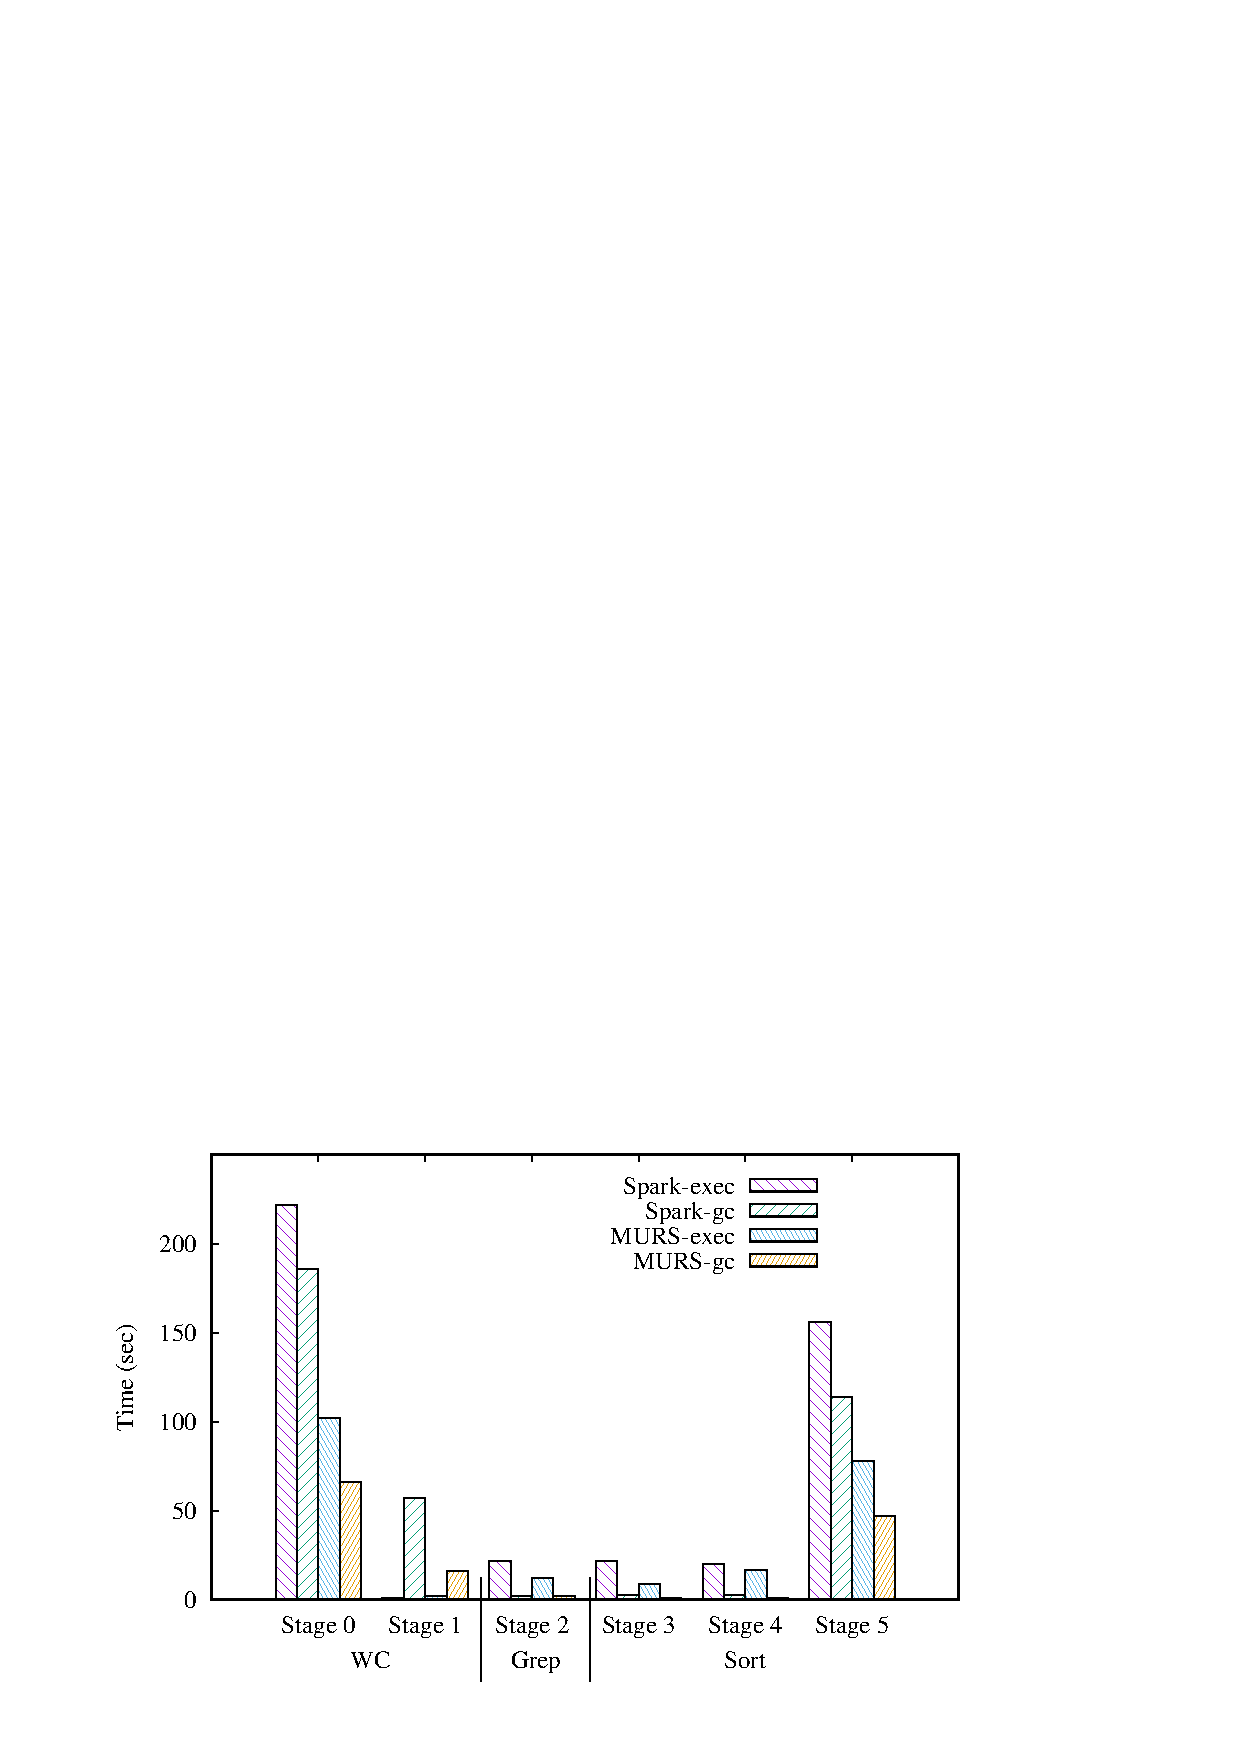
\includegraphics[width=0.4\textwidth]{grep-sort-wc-gc.pdf}
%\vspace{-2mm}
\caption{The Execution and GC Time of Tasks in Sort, Grep and WC}
%\vspace{-4mm}
\label{fig:grep-sort-wc-gc}
\end{figure}

Tasks with constant model in Stage 2 and Stage 3, along with tasks with sub-linear model in Stage 1, all benefit from MURS although the memory pressure is light. This is due to the parallelism in writing to disk, as Spark writes intermediate data in shuffle write phase to disk for checkpoint. Note that when these tasks are running, tasks in Stage 5 have not been launched. MURS is triggered when the proportion of used heap first touch the yellow value, it suspends some tasks in WC and decreases the parallelism in writing to disk. With enough bandwidth of writing to disk, these tasks still execute fast. We find that tasks in Stage 4 benefit less from the parallelism in writing to disk, because they are linear models and suspended by MURS when the proportion of used heap touches the yellow value. 

The reductions of Stage 0 and Stage 5 prove the mitigation on memory pressure through MURS. The garbage collection time in WC has a greater degradation than Sort. While WC suffers heavy memory pressure produced by Sort in Spark, MURS suspends tasks with linear models in Sort and ensures enough memory space for WC. Almost all reduction time comes from the mitigated memory pressure because there are no suspended tasks in WC. Sort gets more memory space after WC completes, and has less memory pressure than Spark. 

%As the Sort application is split into three stages, only tasks in the second stage (this stage just prepares records for the next stage and writes records to disk) and the third stage (this is the actual stage that sorts the key) is the linear model. The function API in the first stage is \textit{flatMap}, which flats the result and provides an iterator, thus it belongs to the constant model. We find that these tasks with sub-linear and linear models suffer greater memory pressure, and all benefit from MURS. However, we can see that the constant model is also a little better, although the garbage collection time has a lower percentage in the original execution time—such as tasks in Grep and the first stage of Sort. This is due to the parallelism in writing to disk. As other tasks suffer heavy memory pressure, MURS stops some tasks and prevents them from writing shuffle data to disk. The accessibility of the disk can be faster, and those running tasks with the constant model can quickly complete their operation on disk. 

\subsection{Memory pressure with caching}

Some frameworks provide caching mechanism for in-memory computation, such as Spark and Flink. Although the in-memory caching data speed up the execution of a job, some works~\cite{bu:bloat, nguyen2015facade} show that it results in greater memory pressure because the caching data live along with the job. Tracing these data is expensive and there is less accessible memory space for execution.

PR is an example of iterative computations that caches important intermediate data in memory. The function API in the first stage of PR is \textit{groupByKey}, which groups all values of the particular key without aggregation. The result of \textit{groupByKey} will be cached in memory and used in subsequent iterations. Thus, the memory usage models of these tasks are linear. Thus, the memory usage models of tasks in Stage 2-3 are linear.  The caching data is alive in memory until the job is completed. Each iteration is implemented in a stage that contains several function APIs: \textit{join}, \textit{map}, and \textit{reduceByKey}. The function APIs \textit{map} and \textit{reduceByKey} are the same as that in Grep and WC. Although \textit{join} distinguishes the key, the function API here just processes the keys in one partition, which means it does not shuffle all keys. Thus, all data objects produced by \textit{join} are temporary data objects, and the sampler will classify it as the constant model. We submit PR along with WC, similarly to Section~\ref{sec:motivation}. The result is shown in Figure~\ref{fig:pr-wc-exec}. We should notice that, when WC job completes, PR is running in Stage 3. During the process of WC, the execution time of WC job is decreased by 28\%, but at the same time the execution time of PR job increased by 26\%. After WC is complete, the execution time of PR job can be decreased by 58\%.

\begin{figure}[!t]
\centering
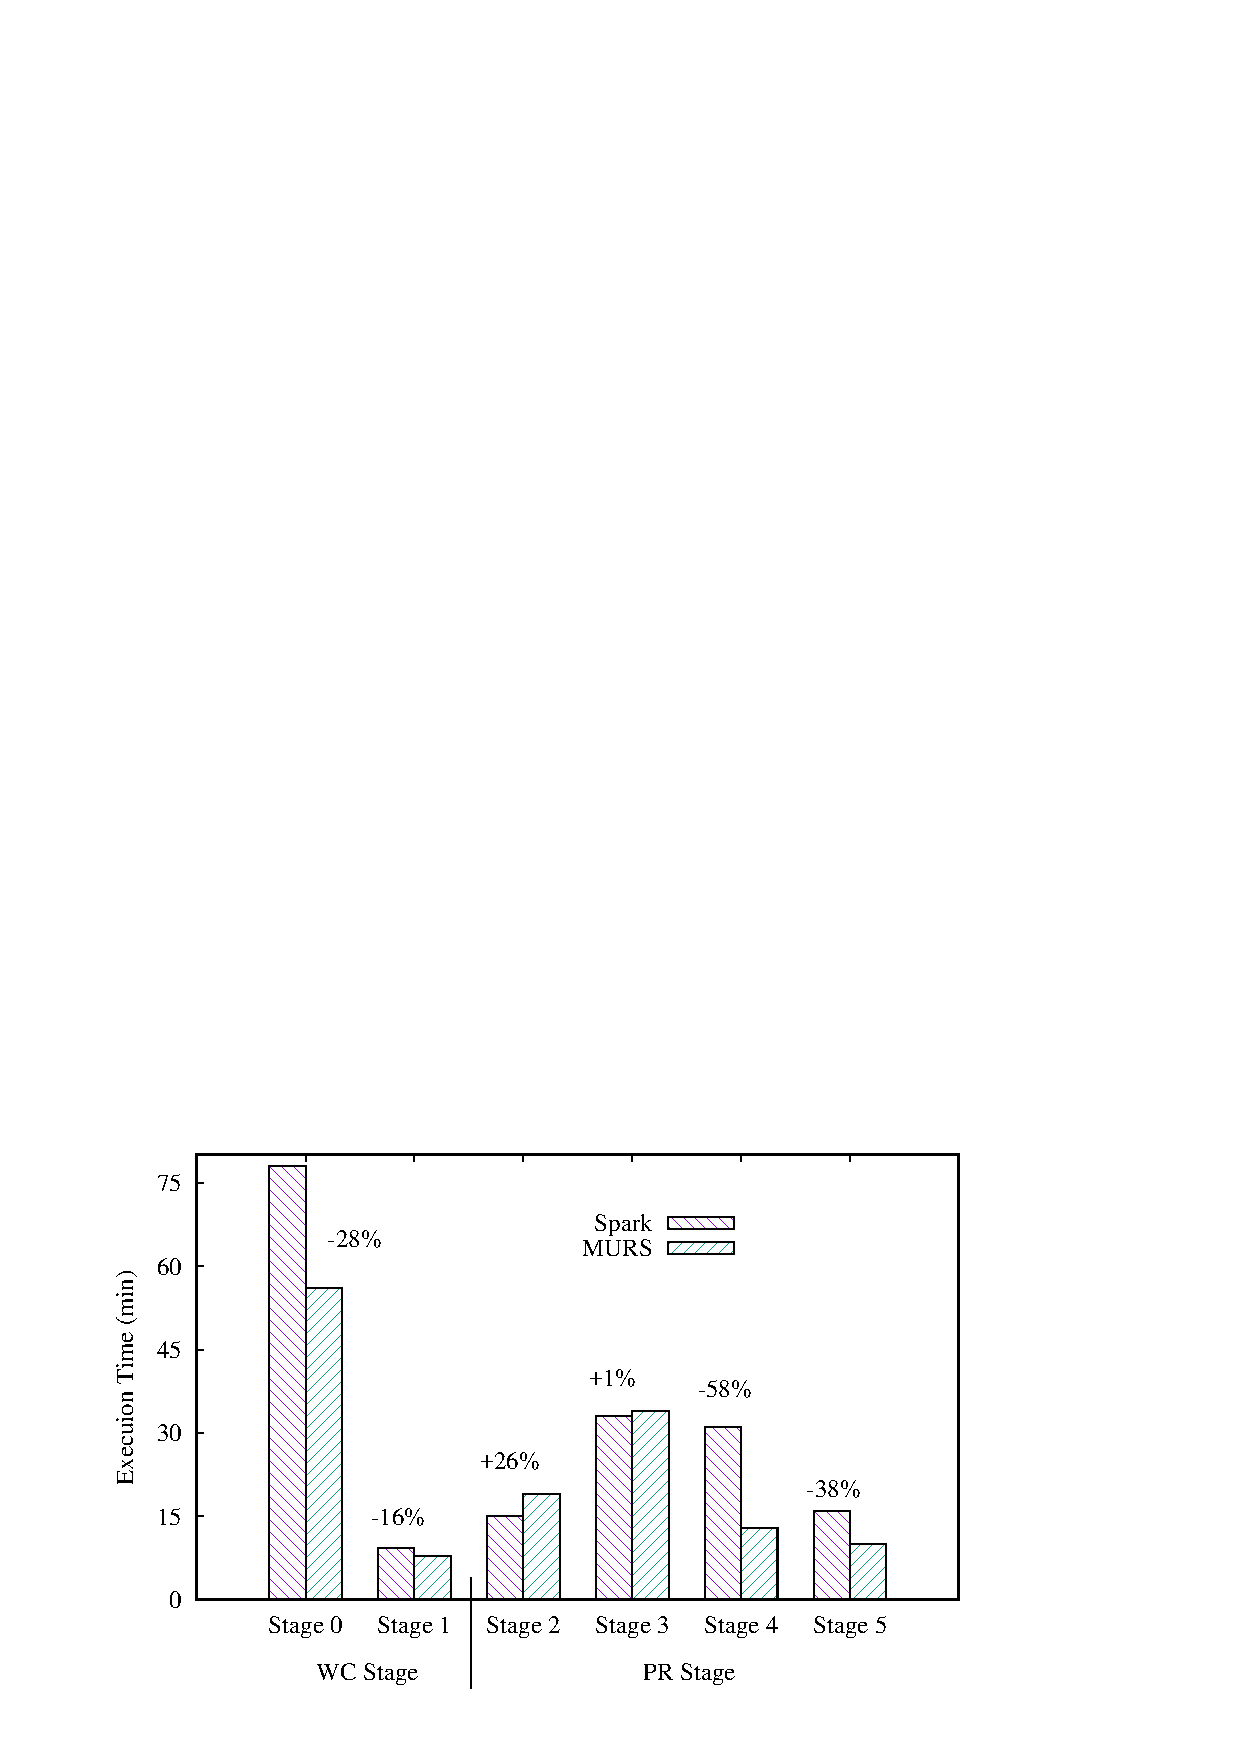
\includegraphics[width=0.4\textwidth]{multitalent-exec.pdf}
%\vspace{-2mm}
\caption{The Execution Time of PR Job and WC Job}
%\vspace{-4mm}
\label{fig:pr-wc-exec}
\end{figure}

\begin{figure}[!t]
\centering
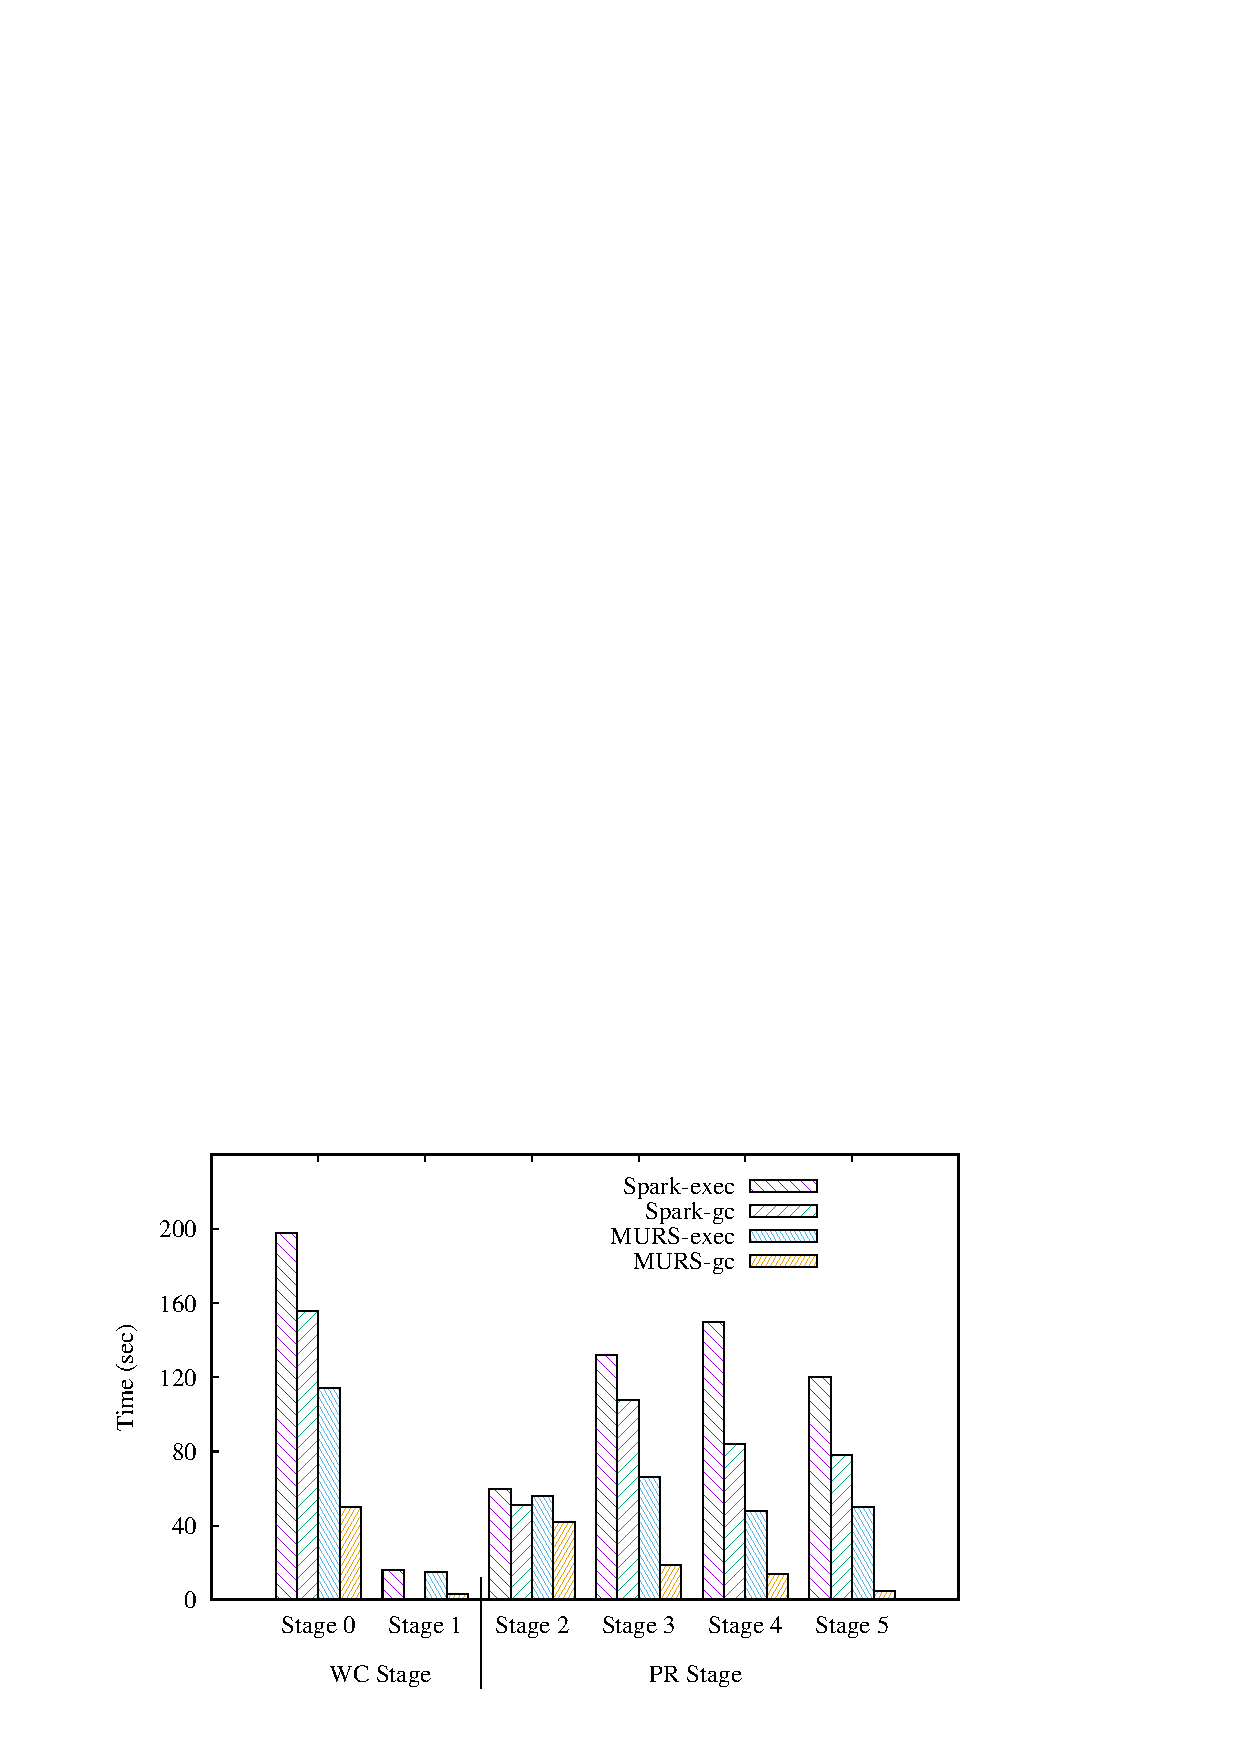
\includegraphics[width=0.4\textwidth]{pr-wc-gc.pdf}
%\vspace{-2mm}
\caption{The Execution and GC Time of Tasks in PR and WC}
%\vspace{-4mm}
\label{fig:pr-wc-gc}
\end{figure}

Before WC completes, tasks in PR and WC both result in memory pressure. However, tasks in PR belong to linear model, while tasks in WC belong to sub-linear model. MURS will suspend these tasks in PR to prevent heavy memory pressure, thus tasks in WC can have a lower execution time.

The execution time of the second stage of PR increases because tasks in PR are always classified to heavy tasks in this scene. In the second stage, PR caches all intermediate data in memory until the job completes. Then the memory manager requires many CPU cycles to trace the caching data objects; and less memory space is accessible for execution, which results in heavy garbage collection. While MURS intends to mitigate the heavy memory pressure, tasks in PR are always classified to heavy tasks because there are no other tasks belong to linear models. Thus, the waiting time of suspended tasks increases greatly although the garbage collection time decreases in Figure~\ref{fig:pr-wc-gc}, and the second stage in PR is even worse in MURS than in Spark for service. Fortunately, as WC completes early, subsequent stages  in MURS suffer much less memory pressure (the garbage collection can be decreased as much as 94\% in some tasks in Figure~\ref{fig:pr-wc-gc}), and performance improves more. 

\subsection{Avoidance of spill}

MURS sets the red value to avoid spill when memory pressure is heavy in these systems who provide spill. We take the evaluation in the last section, which runs PR and WC in the Spark for service, to measure the spill tasks. MURS estimates the size of required memory space for each task, and ensures that running tasks can complete with the remaining memory space. As the estimation is inaccurate to some extent, we find that fewer tasks will still spill in MURS, as shown in Table~\ref{table:spill}. There are no spill tasks in WC in MURS and the spill tasks in PR decreased from 32\% to 2.5\% in comparing to Spark.

\begin{table}[!t]
\small
\centering
\caption{Spill Tasks in MURS and Spark}
\begin{tabular}{| c | c | c | c | c | c | c | c |}

\hline
\multirow{2}{*}{} & \multirow{2}{*}{\textbf{App}} & \multicolumn{3}{| c |}{\textbf{Spill Percentage}} & \multicolumn{3}{| c |}{\textbf{Spill Size (MB)}} \\
\cline{3-8}
 & & total & spill & percent & min & mid & max \\
\hline
\multirow{2}{*}{Spark} & WC & 1000 & 91 & 9\% & 0 & 0 & 710 \\
\cline{2-8}
 & PR & 1500 & 480 & 32\% & 310 & 367 & 439 \\
\hline
\multirow{2}{*}{MURS} & WC & 1000 & 0 & 0\% & - & - & -  \\
\cline{2-8}
 & PR & 1500 & 37 & 2.5\% & 0 & 0 & 458 \\
\hline

\hline
\end{tabular}
%\vspace{-2mm}
 
%\vspace{-6mm}
\label{table:spill}
\end{table}

We should acknowledge that error exists in the avoidance of spill. The sampler in MURS counts two important metrics of one task: the percentage of processed records in total records, and the current allocated memory space for this task. We can quickly get the required memory space based on these two metrics. When memory pressure reaches the red value, we suspend parts of tasks and leave enough remaining memory space for running tasks. As the estimate is based on sampling, error exists in the estimated size of allocated memory space, especially when the value in some key-value pairs is a collection. Different records have different sizes because the number of values inside a collection is different, such as \textit{groupByKey} in PR. Some hot keys may result in substantial error. Thus, it can be accepted that there are even fewer spill tasks in MURS.

\subsection{Memory pressure in multi-launch}

Some systems for service are oversold and launches multiple tasks than the original configuration. When the service is idle, it has efficient memory usage. However, if the service comes to busy, the memory pressure is uncontrollable and the performance will degrade quickly when memory pressure is heavy. MURS is appropriate for this problem as it keeps the advantage in light memory pressure but prevents memory pressure increasing fast in heavy memory pressure. We choose WC here and two datasets to compare the impact of multi-launch MURS with Spark. We submit WC independently here to clearly distinguish the light and heavy memory pressure, and MURS can also work as mentioned in Section~\ref{sec:desgin}. WC processes data as (\textit{K}, \textit{V}), while \textit{K} means the words in the dataset. Thus, the number of words will decide the size of shuffle buffer, and more words will result in more memory pressure. As shown in Figure~\ref{fig:subfig:wc-million}, the GC time can be increased to 31.8\%, but the reduction of execution time is 11.6\% when the number of words is 1 million; the reduction of execution time is 22.9\% and the GC time can be 45.2\% when the number of words increases to 100 million in Figure~\ref{fig:subfig:wc-billion}.

%Although MURS is designed for data processing systems for service, we find it can also work well in batch processing when all running tasks have the same model. We choose WC here and two datasets to compare the impact of multi-launch in different memory pressures. WC process data as (\textit{K}, \textit{V}), while \textit{K} means the words in the dataset. Thus, the number of words will decide the size of shuffle buffer, and more words will result in more memory pressure. As shown in Figure~\ref{fig:subfig:wc-million}, the GC time can be increased to 31.8\%, but the reduction of execution time is 11.6\% when the number of words is 1 million; the reduction of execution time is 22.9\% and the GC time can be 45.2\% when the number of words increases to 1 billion in Figure~\ref{fig:subfig:wc-billion}.

\begin{figure}[!t]
\centering
\subfigure[Light memmory pressure]{
\label{fig:subfig:wc-million}
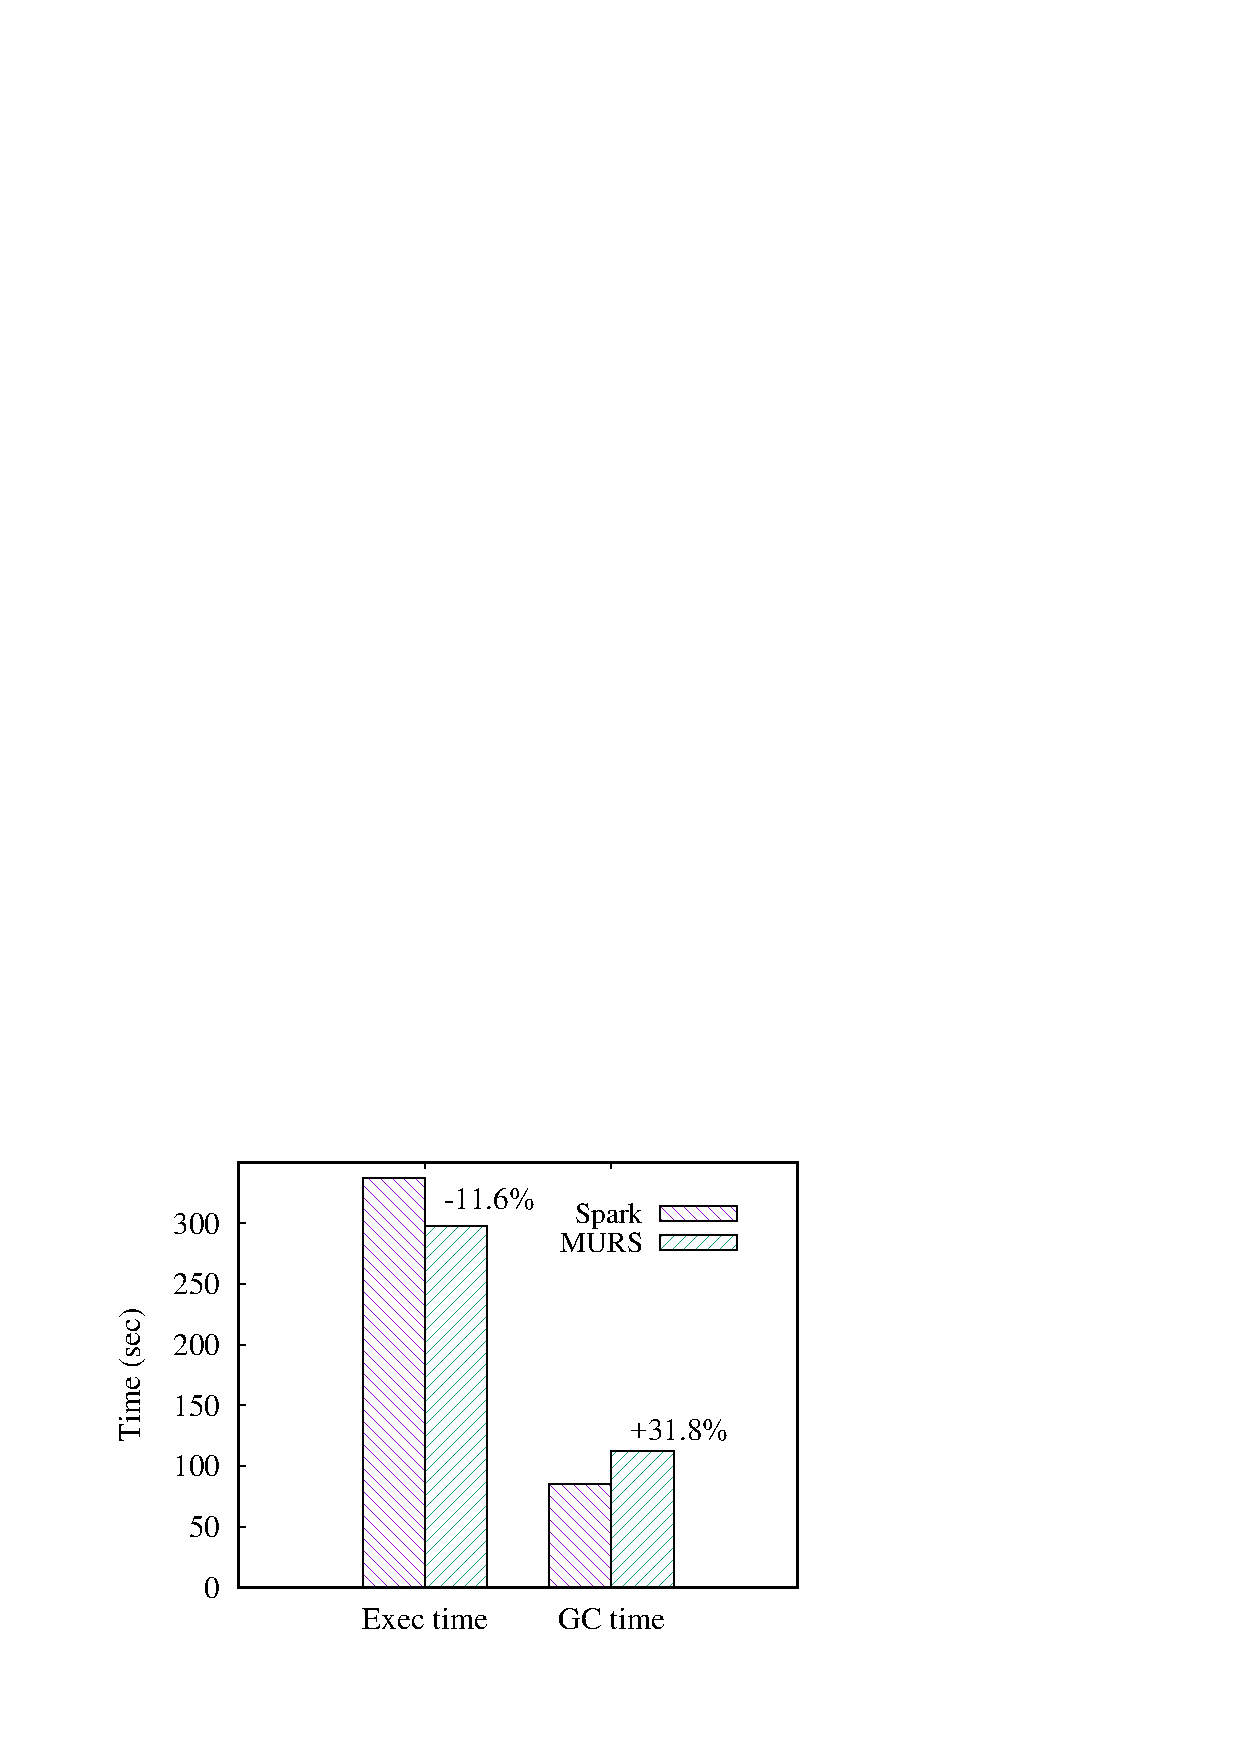
\includegraphics[width=0.231\textwidth]{wc-million.pdf}}
\hspace{-1.3ex}
\subfigure[Heavy memory pressure]{
\label{fig:subfig:wc-billion}
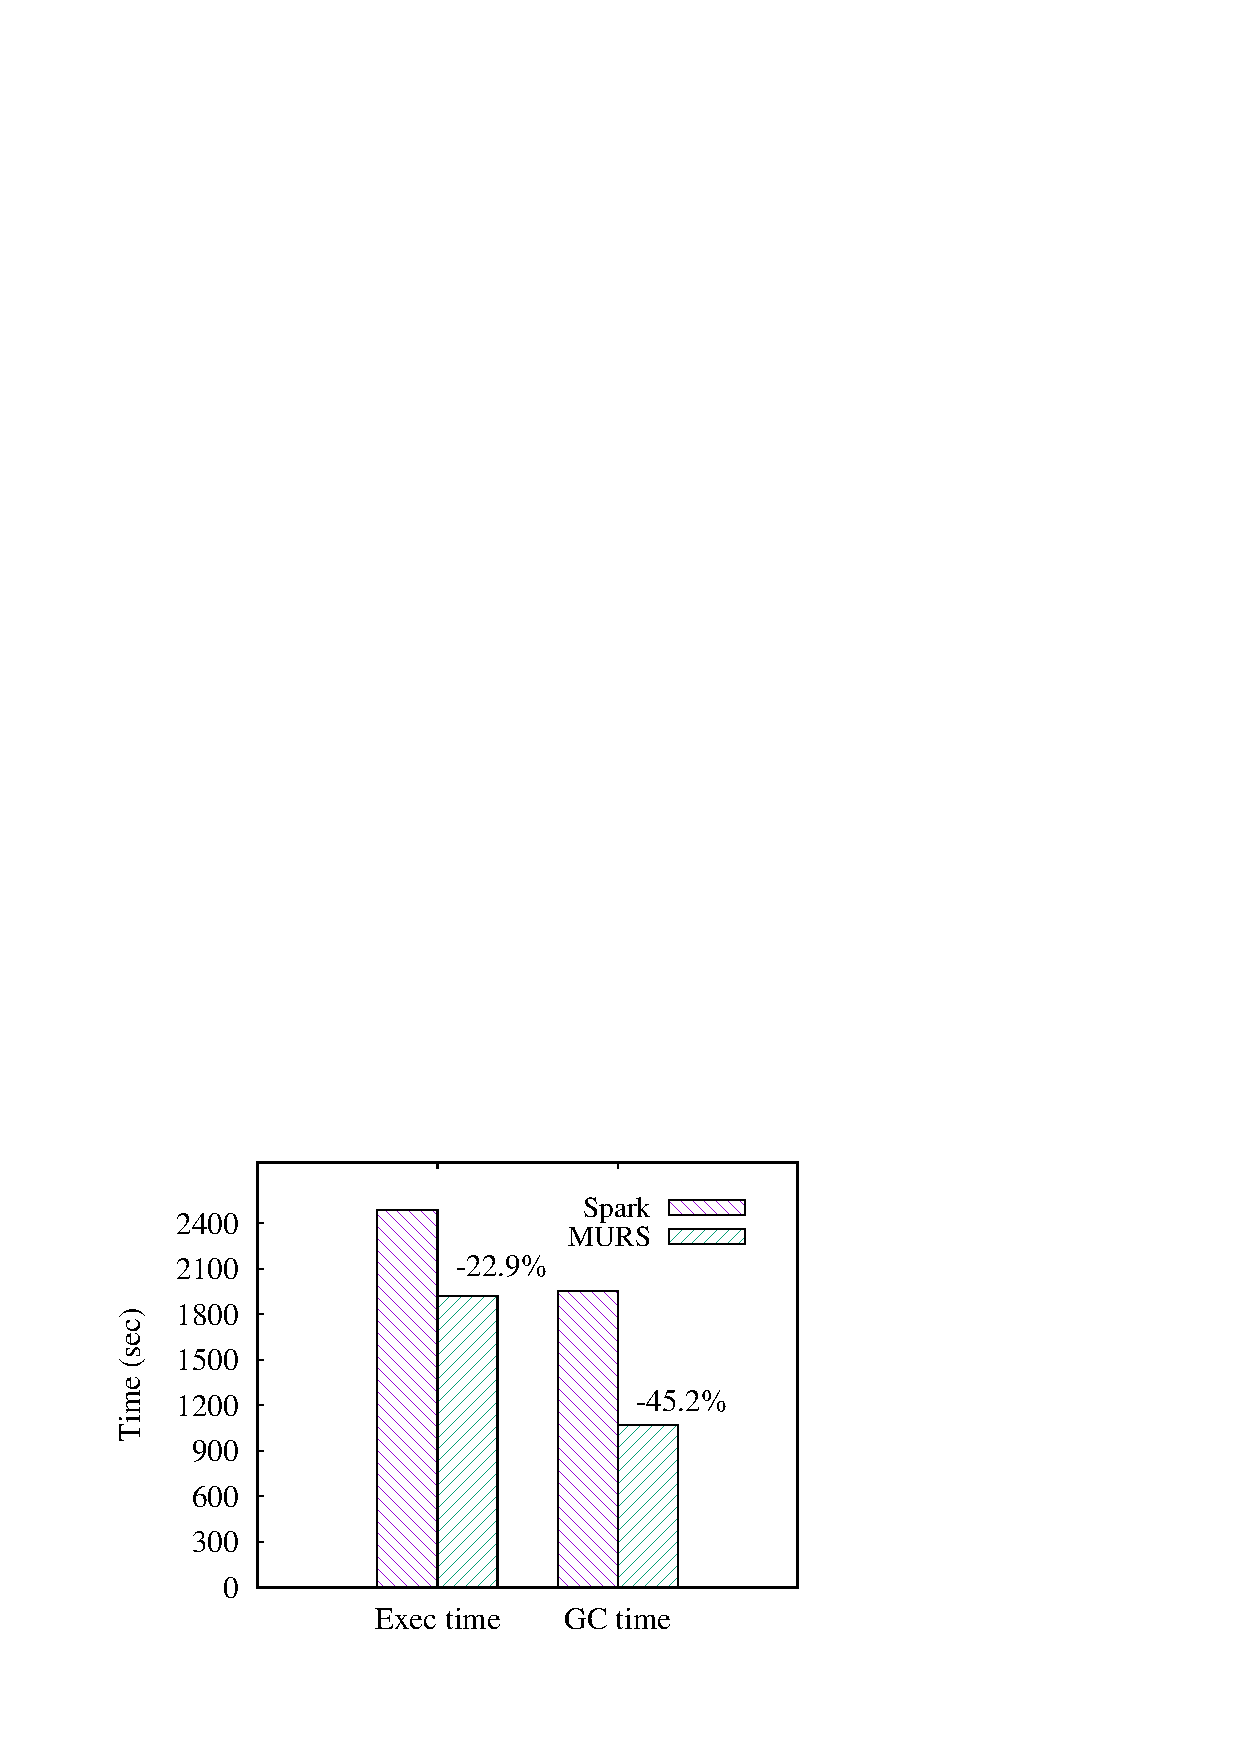
\includegraphics[width=0.231\textwidth]{wc-billion.pdf}}
\label{fig:wc-result}
%\vspace{-2mm}
\caption{Multi-launch with MURS when service is busy}
%\vspace{-4mm}
\end{figure}

Light memory pressure usually means that memory space will suffer less allocation and reclamation. Multi-launch increases the parallelism as well as the memory pressure, which properly increase the frequency of memory allocation and reclamation. This improves the efficiency of memory usage. Thus the services work well with multi-launch in Figure~\ref{fig:subfig:wc-million}. MURS remains the advantages in this scene. However, when the words increases to 100 million, memory pressure is high and the throughout is only 25.6\%. Frequent garbage collection degrades the performance quickly. MURS will suspend numbers of tasks to prevent the increase of memory pressure, thus both execution time and garbage collection time decrease in Figure~\ref{fig:subfig:wc-billion}.



















\begin{comment}

\subsection{Batch Processing}

\subsubsection{Impcat of Shuffle Function}
WordCount in Spark benchmark is an original MapReduce application. WC has two stages: the first stage reads data from HDFS and writes shuffle buffers; the second stage reads data from shuffle buffers and then function \textit{reduceByKey} is used to get the result. Shuffle buffers process data as (\textit{Key},\textit{Value}) while \textit{Key} means the words in dataset. Thus the number of words will decide the size of shuffle buffers, and more words will result in more memory pressure. As shown in Figure~\ref{fig:subfig:wc-million}, the GC time can be increased to 31.8\% but the reduction of execution time is 11.6\% when the number of words is 1 million; the reduction of execution time is 22.9\% and the GC time can be 45.2\% when the number of words increases to 1 billion in Figure~\ref{fig:subfig:wc-billion}.

When the size of words is small, the shuffle buffers will have less keys. The size of shuffle buffers will not result in heavy memory pressure which can also be proved by the light garbage collection. MURS provides multi launch to increase the memory pressure and parallelism of job, the running tasks is 1.5x than Spark. Thus the execution time decreases but the garbage collection time increases in Figure~\ref{fig:subfig:wc-million}. However, when the words increases to 1 billion, memory pressure can be high and the throughout is only 25.6\%. MURS will stop numbers of tasks to prevent the increase of memory pressure and both execution time and garbage collection time will decrease in Figure~\ref{fig:subfig:wc-billion}. 

\subsubsection{Impcat of Caching and Shuffle Function}
PageRank(PR) will firstly cache important intermediate data of function \textit{groupByKey} in memory. Each of the appending several iterations is a stage in the job. The main functions in each stage are \textit{join} and \textit{reduceByKey}. The function \textit{join} not belongs to shuffle function in PR. We test 10 iterations here and the result is shown in Figure~\ref{fig:pr-stagetime}. While the first stage just read data from HDFS, the memory pressure is light. After stages will suffer from caching data in memory. The size of caching data in each node is 4.1GB-5.3GB. Different stage has different memory pressure, the max execution time has the speed up of 2.1x to the min in Spark. Different memory pressure and tasks result in different performance of MURS. The best reduction of execution time can be 56\% and the average reduction is 44\% for computing stages.

\begin{figure}[!t]
\centering
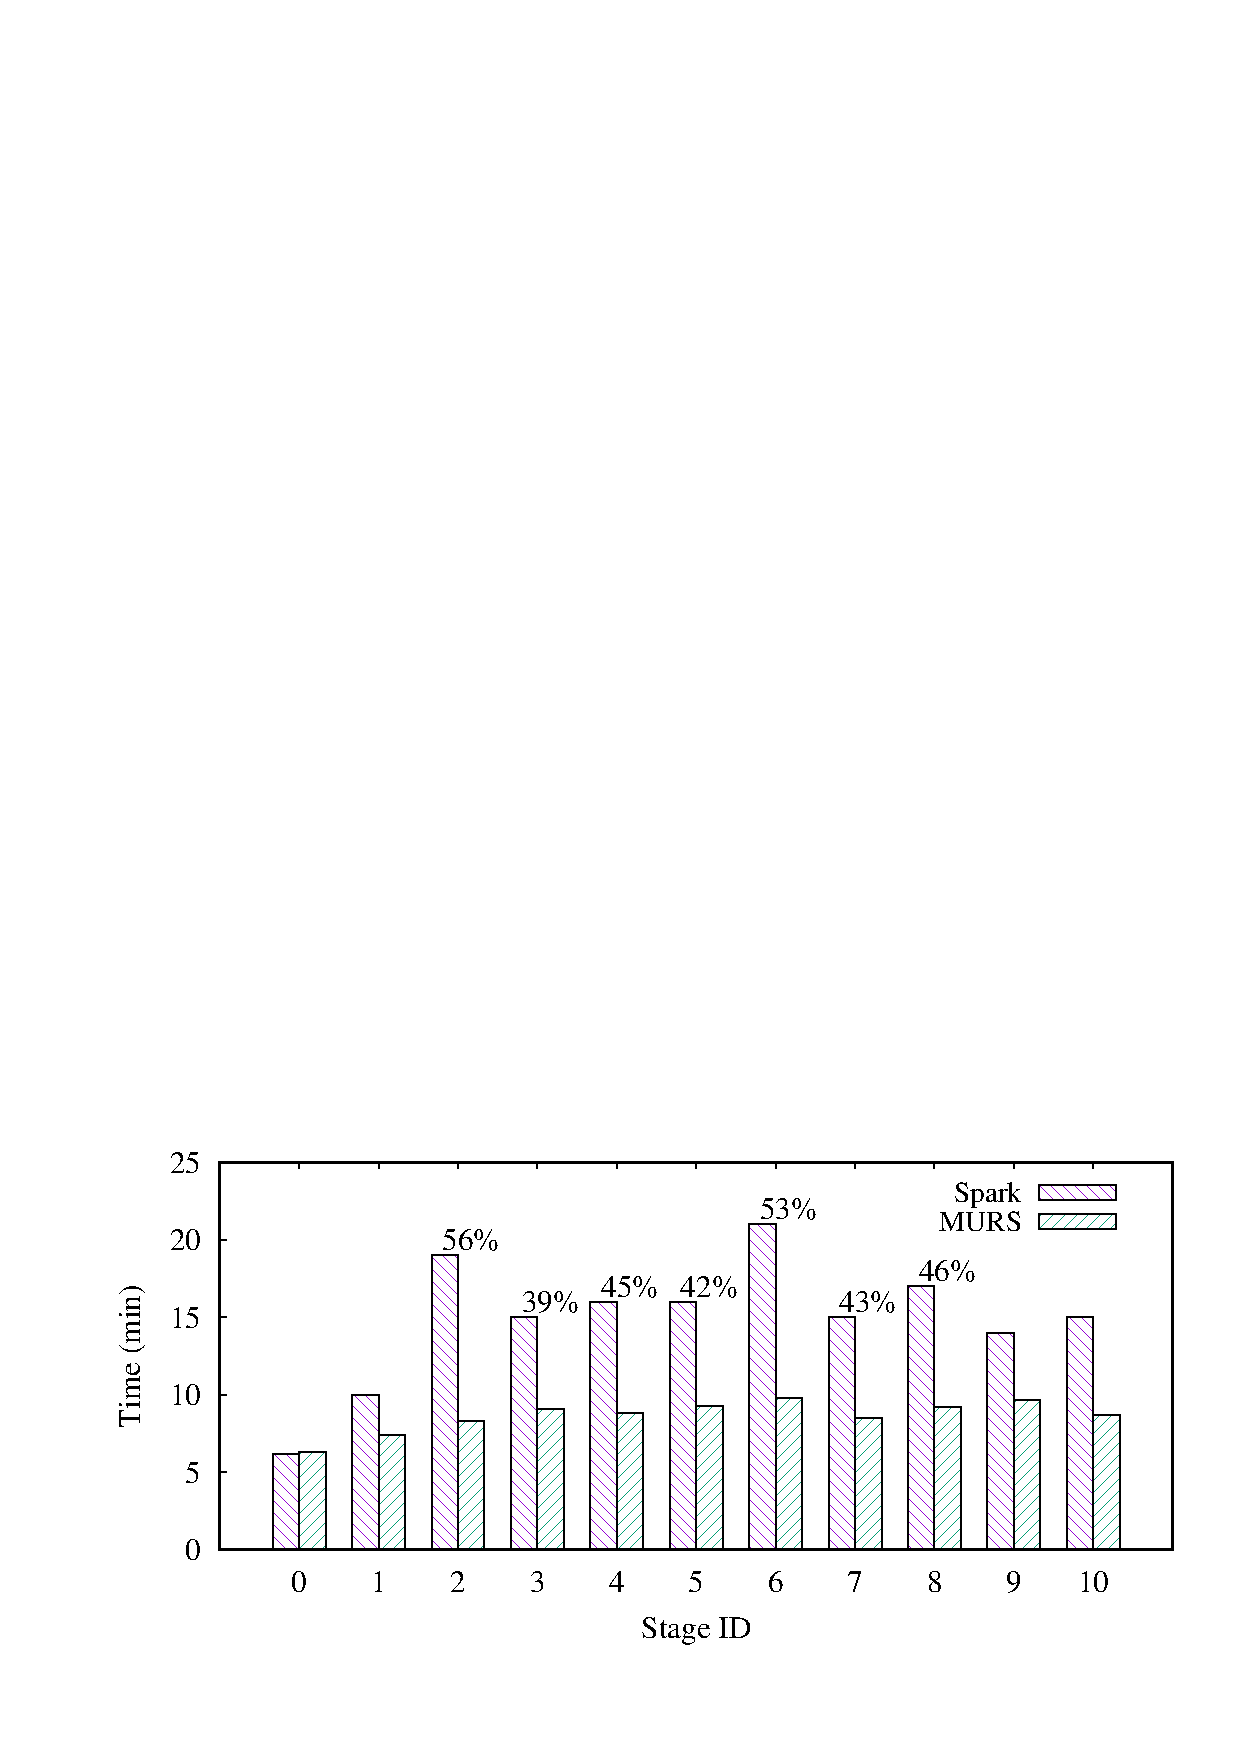
\includegraphics[width=0.45\textwidth]{pr-stagetime.pdf}
\vspace{-2mm}
\caption{The Result of Each Stages in PageRank}
\vspace{-2mm}
\label{fig:pr-stagetime}
\end{figure}

The caching data cost constant memory space because the caching data has same lifetime in the job. While less execution memory space is accessible for shuffle operation, the same data objects will result in worse memory pressure and more frequently garbage collection. The improvement of PageRank in MURS is benefit from three points: GC reduction, spill avoidance  and stopping tasks.

\begin{figure}[!t]
\centering
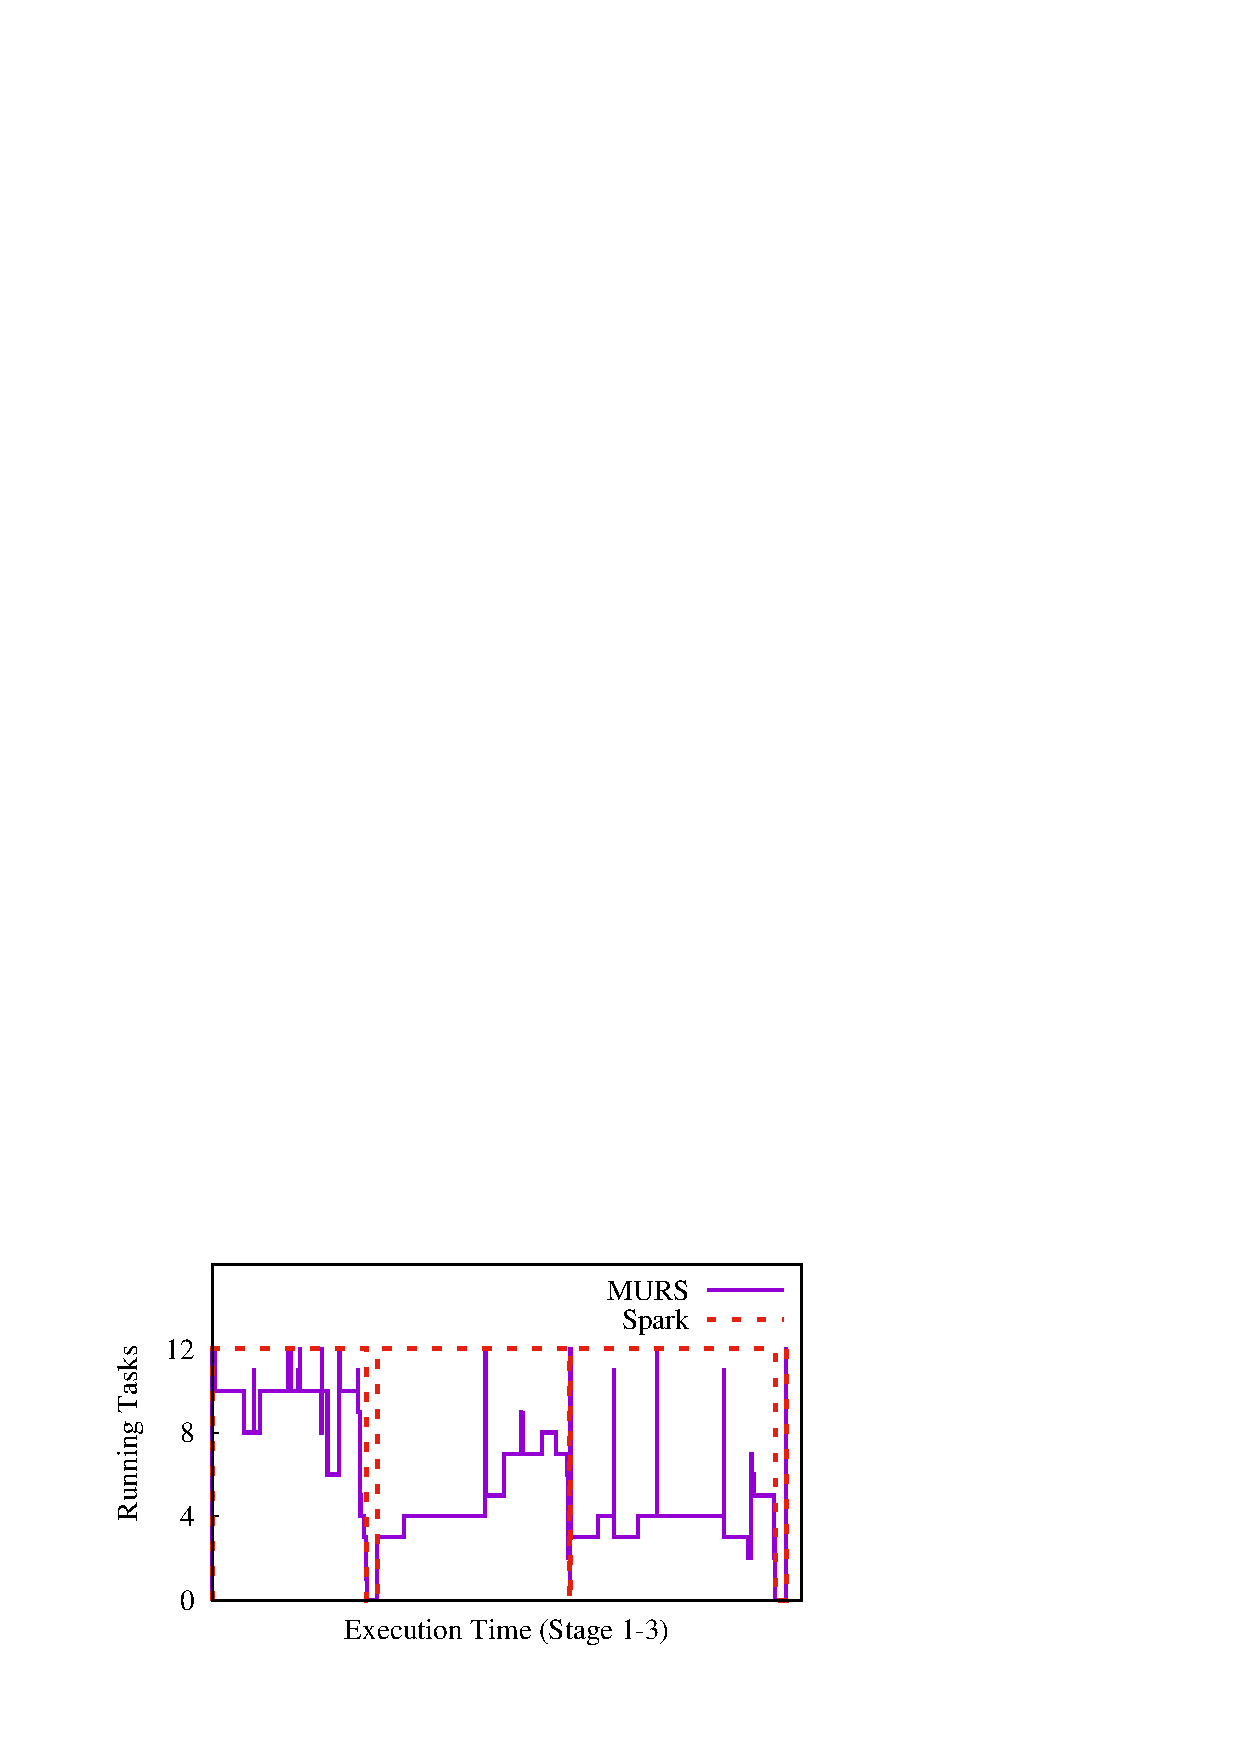
\includegraphics[width=0.35\textwidth]{pr-runtasks.pdf}
\vspace{-2mm}
\caption{The Number of Running Tasks in MURS}
\vspace{-2mm}
\label{fig:pr-runtasks}
\end{figure}

\textbf{Stopping tasks} The core scheduling in MURS is stopping parts of tasks to prevent heavy memory pressure, thus we firstly analysis the count of running tasks as shown in Figure~\ref{fig:pr-runtasks}. The first stage has no caching data but some shuffle buffers in memory. The shuffle buffer will be live in JVM heap until write to disk, thus they result in some memory pressure and our scheduler stop two tasks accordingly. When the job runs in after stages, caching data will stay in memory until the job complete. The heavy memory pressure result in more stopped tasks.

\begin{figure}[!t]
\centering
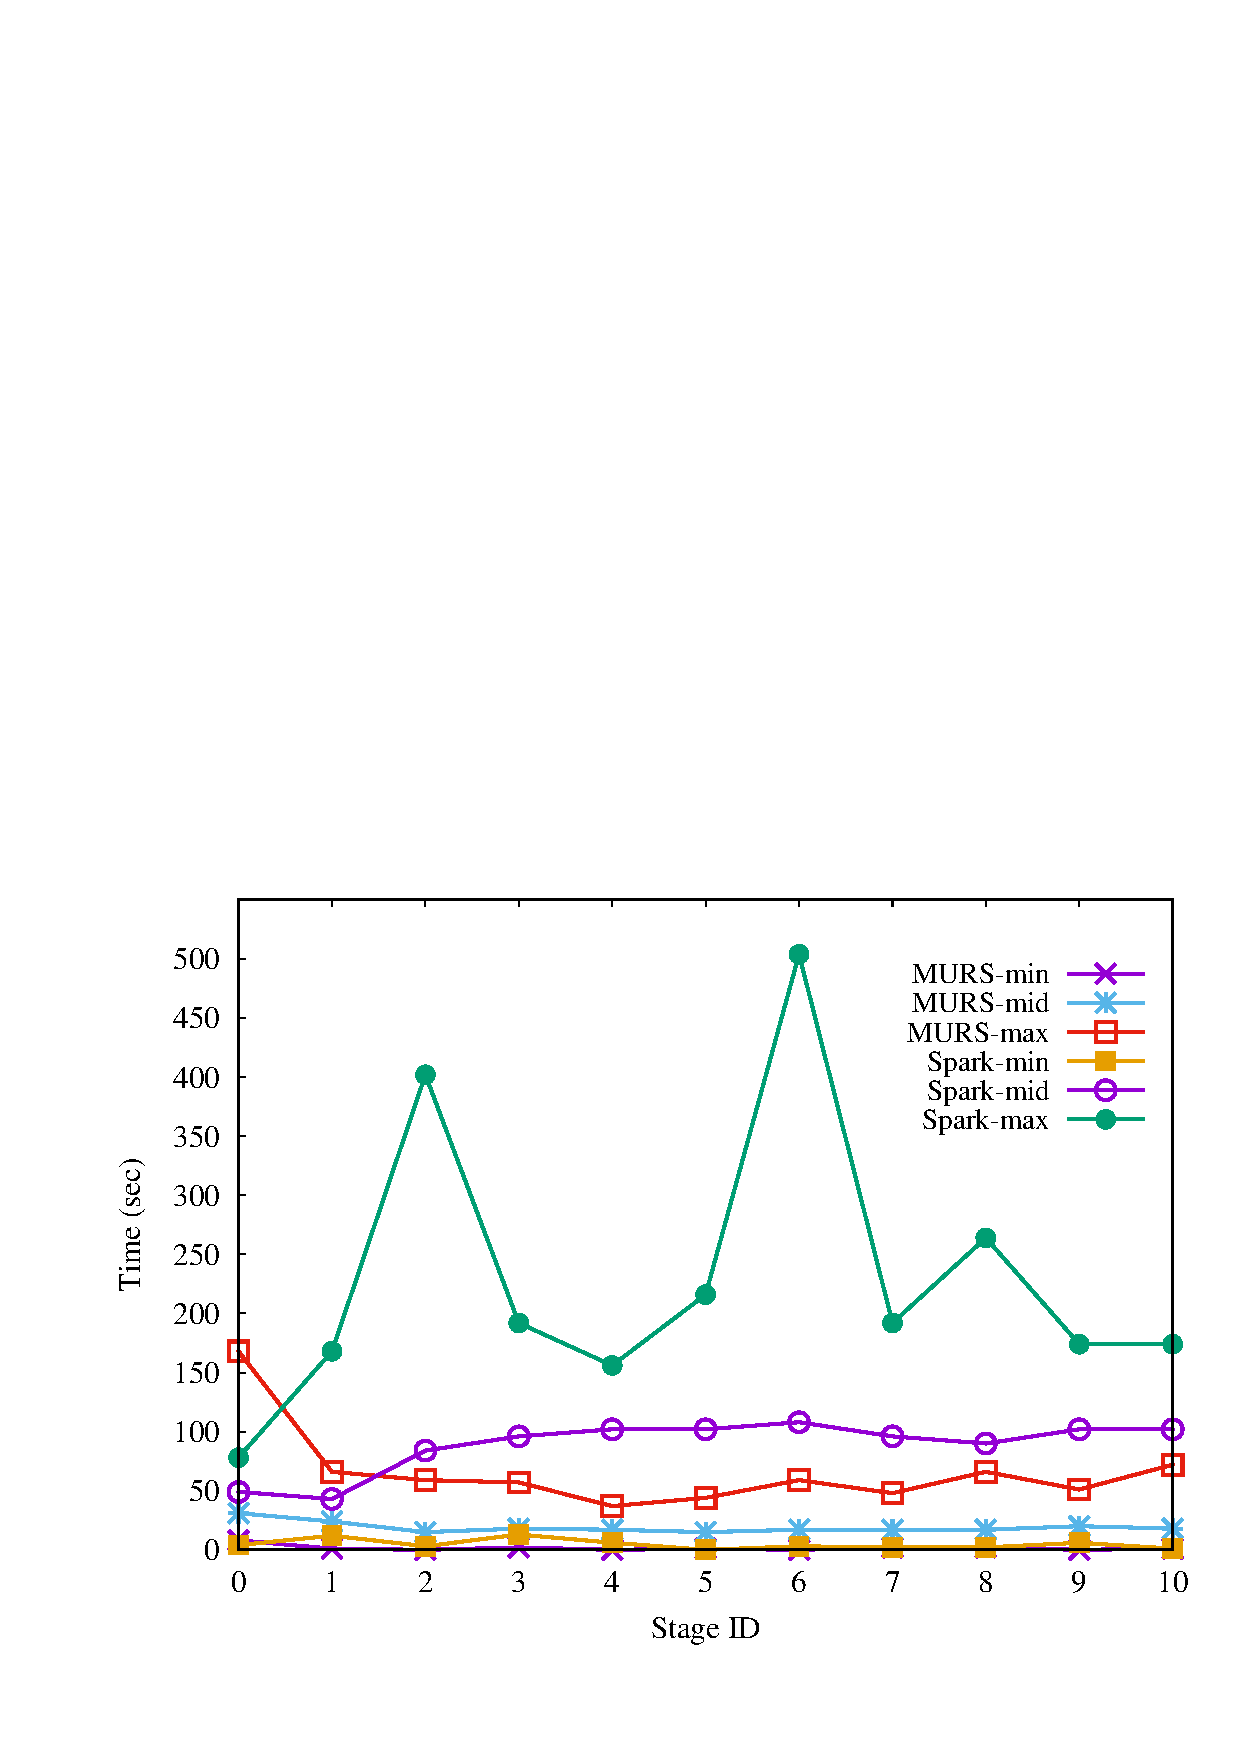
\includegraphics[width=0.45\textwidth]{pr-gc.pdf}
\vspace{-2mm}
\caption{The GC of Total Tasks in PageRank}
\vspace{-4mm}
\label{fig:pr-gc}
\end{figure}

\textbf{GC reduction} Each task suffers from different garbage collection, as shown in Figure~\ref{fig:pr-gc}. We compare the minimum, median and maximum of total tasks. Each guideline in MURS is better than Spark. The median of garbage collection time in MURS has the speed up of 5.5x. The reduction of garbage collection can be more cleared with the peak execution memory of each task. Peak execution memory of each task is 457MB/533MB/868MB(min/mid/max) in MURS, and 369MB/493MB/597MB(min/mid/max) in Spark. As MURS stop some tasks to avoid the cost of memory space which will be occupied for a long time, other running tasks has more execution memory. While the same memory space is provided for less running tasks, the peak execution memory of each tasks will be high. If the peak execution memory is high, tasks can run without heavy memory pressure because less garbage collection will occur. After the running tasks release their occupied space, stopped tasks can also improve their peak execution memory. Thus the memory pressure in MURS is lighter than Spark, and more execution memory slow down the heavy garbage collection essentially.

We can also get the conclusion that the straggler can be avoided in some way. The max garbage collection time and the average time is much near in MURS but fluctuating serious in Spark. As the time of garbage collection makes up the important part of execution time, tasks with long period of garbage collection will have long execution time. If the execution time of one task exceeds the average time of completed tasks, we regard it as an straggler. Thus MURS will have low probability to produce the straggler.

\begin{table}[!t]
\small
\centering
\begin{tabular}{| c | c | c | c | c | c | c | c |}

\hline
\multirow{2}{*}{} & \multirow{2}{*}{Stage} & \multicolumn{3}{| c |}{Spill Percent} & \multicolumn{3}{| c |}{Spill Size (MB)} \\
\cline{3-8}
 & & total & spill & percent & min & mid & max \\
\hline
\multirow{2}{*}{Spark} & stage6 & 300 & 185 & 62\% & 0 & 370 & 480 \\
\cline{2-8}
 & stage1 & 300 & 52 & 17\% & 0 & 0 & 471 \\
\hline
\multirow{2}{*}{MURS} & stage6 & 300 & 0 & 0\% & - & - & -  \\
\cline{2-8}
 & stage1 & 300 & 1 & 1\% & 0 & 0 & 399 \\
\hline

\hline
\end{tabular}
\vspace{-2mm}
\caption{Spill Tasks in MURS and Spark} 
\vspace{-4mm}
\label{table:pr-spill}
\end{table}

\textbf{Spill avoidance} Spark has several spill tasks in each stage, and only one stage of MURS has spill tasks, as shown in Table~\ref{table:pr-spill}. No matter in the first stage or other stages, most tasks can avoid spilling in MURS although they would spill in Spark. The fundamental reason is also more execution memory. MURS has the spill computing algorithm to avoid spilling. After stopping tasks, remain space are enough to running tasks is just the goal of MURS. While multi launch is available, the spill computing algorithm is more functional to control the running tasks. We notice that spill also appear in MURS, there are two points here: 1) estimating the remaining using space of one running task is not usually accurate; 2) the available memory space of one thread in JVM is limited (1/2N at least and 1/N at most while N is the number of running threads in JVM). Spill can result in expensive disk IO, thus the performance can be better.% in MURS.

\subsection{Multi-tenant}

Spark JobServer can provide multi-tenant for Spark. We submit both WordCount and PageRank to the Spark JobServer to test the performance of MURS in multi-tenant. We set the number of iterations to be 3 in PageRank, when the WordCount completes, PageRank usually complete the second stage. The result is shown in Figure~\ref{fig:mul-exec}. The execution time of WordCount decreased 28\% but at the same time the execution time of PageRank increased 26\%. After WordCount is complete, the execution of PageRank can be decreased to 58\%. We should notice that, when the WordCount is complete the PageRank runs both in Stage 2.

In the first stage, tasks in PR and WC are both \textit{ShuffleMapTask} which result in memory pressure through the shuffle buffer in shuffle writer. However, the function APIs in PR is \textit{groupBykey} which is a non-aggregation, it increases the size of shuffle buffer for each processed record. The function APIs in WC is \textit{reduceByKey} which is an aggregation, it increases the size of shuffle buffer only when the \textit{K} of processed record has never appeared. Obviously, the tasks in PR belong to linear while the tasks in WC belong to sub-linear. Our scheduler will stop the tasks of PR to prevent the heavy memory pressure, thus the tasks of WC can have less execution time. The pity is that the waiting time of stopped tasks increased much. Fortunately, as WC completes early, the third stage (Stage 2) in MURS suffer much less memory pressure, and the performance improves more. This is much important in multi-tenant, not only the tasks with heavy influence on memory pressure can execute more quickly, but also these tasks with light influence can avoid the memory pressure. The service of all tenant, which means PR and WC, can be better.

\end{comment}



\section{Related Work}

The problem of memory pressure in a system has been studied for several years. Different methods have been proposed to address this issue, such as tuning of garbage collection, memory management and task scheduling. Most of these works focus on the offline calculation in data processing systems. 

\textbf{Garbage Collection} Most methods of garbage collection tuning are based on the features of different applications, such as Spark applications~\cite{www:spark-tuning}, Cassandra applications~\cite{www:cassandra}. These methods typically take the following two approaches: 1) replacing other garbage collection algorithms, such as Concurrent Mark Sweep (CMS) or Garbage First (G1), 2) tuning the important parameters, such as the ratio of young generation and old generation, to avoid frequent GC activity and data copying. Most researches attempt to rebuild the algorithm of garbage collection for common applications. For example, Yang et al.\cite{yang:fullgc} describes an incremental query model for reference calculations to optimize the cause of full GC. This garbage collection algorithm is universally useful to most memory pressure cases. Rodrigo et al.\cite{rodigo:NGeneration} proposed a N-Generational garbage collector for big data memory management, which also reduces the data copying in garbage collection. Tuning garbage collection requires the deep understanding and proficient skills on the data processing systems.

\textbf{Memory Management} The memory analysis of data-intensive big data applications are put forward by Bu et al.~\cite{bu:bloat}. They consider the bloat of memory in object-oriented languages and design the bloat-aware paradigm: 1) merging small data to big data; 2) manipulating the data by directly accessing the buffers. Some memory management techniques at the system level also extend the language-level optimization, such as region based memory management (RBMM)~\cite{nguyen2015facade, nguyen:yak} and lifetime based memory management~\cite{lulu:deca}. Nguyen et al.~\cite{nguyen2015facade} advise the users to mark the class information in the applications to decompose the data object to regions. Then the memory can be allocated or reclaimed by the regions. Based on the same theory, they also proposed a new garbage collector to mange the data objects and control the objects separately to extend the method to iterative computations~\cite{nguyen:yak}. Lu et al.~\cite{lulu:deca} propose the lifetime-based memory management. They decompose the data objects based on the data container, which decides the lifetime of data objects. The decomposed data objects will impose less pressure on the memory and can be allocated and reclaimed by regions. Memory management provides an effective way to manage the memory pressure and has been investigated by a large body of research.

\textbf{Task Scheduler} As the memory pressure is caused by the running tasks, the task scheduler can also play a role in releasing the memory pressure or improving the efficiency of memory usage. Fang et al.~\cite{fang2015interruptible} design the interruptible tasks for data-parallel programs. They classify the memory consumption of a task into four parts: local data structures, processed input, unprocessed input and result. Based on their novel programming model, suspending the interruptible tasks can release parts of the memory consumption of random tasks when memory pressure mounts. The suspended tasks can be resumed when memory pressure decreases. 
%Interruptible tasks can be resumed with the remaining in-memory data. 
Pu et al.~\cite{pu2016fairride} implement a new policy called FairRide, which  is able to fairly allocate the memory cache to multiple users with the shared files through the efficient blocking. This policy is the first to satisfy all three desirable properties: isolation-guarantee, strategy-proofness and Pareto-efficiency. Based on different scheduling standards, the task scheduler always adapts to different demands and is easy to be implemented.

\section{Conclusion}

In order to mitigate the memory pressure in current data processing systems deployed as the services, we analyze the memory usage of various function APIs enclosed in these systems, and build four coarse-grained models to classify the function APIs. Further, we propose to use the memory usage rate as a uniform criteria to measure the impact of a task on memory pressure. In this paper, we develop a scheduler called MURS, which is based on the memory usage rate. MURS can suspend the tasks that cause heave memory pressure, and speed up the tasks with light memory pressure. MURS can be implemented in most data processing systems. We conducted extensive experiments to evaluate the effectiveness of the proposed methods. The results show that Comparing with Spark, MURS can reduce the execution time of tasks by up to 65.8\%, mitigate the memory pressure by up to 81\% and avoid the task spill by approximately 90\%.

%\section{Introduction}
% no \IEEEPARstart
%This demo file is intended to serve as a ``starter file''
%for IEEE conference papers produced under \LaTeX\ using
%IEEEtran.cls version 1.7 and later.

%All manuscripts must be in English. These guidelines include complete descriptions of the fonts, spacing, and related information for producing your proceedings manuscripts. Please follow them and if you have any questions, direct them to the production editor in charge of your proceedings at Conference Publishing Services (CPS): Phone +1 (714) 821-8380 or Fax +1 (714) 761-1784.
% You must have at least 2 lines in the paragraph with the drop letter
% (should never be an issue)

%\subsection{Subsection Heading Here}
%Subsection text here.


%\subsubsection{Subsubsection Heading Here}
%Subsubsection text here.

%\section{Type style and Fonts}
%Wherever Times is specified, Times Roman or Times New Roman may be used. If neither is available on your system, please use the font closest in appearance to Times. Avoid using bit-mapped fonts if possible. True-Type 1 or Open Type fonts are preferred. Please embed symbol fonts, as well, for math, etc.


% An example of a floating figure using the graphicx package.
% Note that \label must occur AFTER (or within) \caption.
% For figures, \caption should occur after the \includegraphics.
% Note that IEEEtran v1.7 and later has special internal code that
% is designed to preserve the operation of \label within \caption
% even when the captionsoff option is in effect. However, because
% of issues like this, it may be the safest practice to put all your
% \label just after \caption rather than within \caption{}.
%
% Reminder: the "draftcls" or "draftclsnofoot", not "draft", class
% option should be used if it is desired that the figures are to be
% displayed while in draft mode.
%
%\begin{figure}[!t]
%\centering
%\includegraphics[width=2.5in]{myfigure}
% where an .eps filename suffix will be assumed under latex, 
% and a .pdf suffix will be assumed for pdflatex; or what has been declared
% via \DeclareGraphicsExtensions.
%\caption{Simulation Results}
%\label{fig_sim}
%\end{figure}

% Note that IEEE typically puts floats only at the top, even when this
% results in a large percentage of a column being occupied by floats.


% An example of a double column floating figure using two subfigures.
% (The subfig.sty package must be loaded for this to work.)
% The subfigure \label commands are set within each subfloat command, the
% \label for the overall figure must come after \caption.
% \hfil must be used as a separator to get equal spacing.
% The subfigure.sty package works much the same way, except \subfigure is
% used instead of \subfloat.
%
%\begin{figure*}[!t]
%\centerline{\subfloat[Case I]\includegraphics[width=2.5in]{subfigcase1}%
%\label{fig_first_case}}
%\hfil
%\subfloat[Case II]{\includegraphics[width=2.5in]{subfigcase2}%
%\label{fig_second_case}}}
%\caption{Simulation results}
%\label{fig_sim}
%\end{figure*}
%
% Note that often IEEE papers with subfigures do not employ subfigure
% captions (using the optional argument to \subfloat), but instead will
% reference/describe all of them (a), (b), etc., within the main caption.


% An example of a floating table. Note that, for IEEE style tables, the 
% \caption command should come BEFORE the table. Table text will default to
% \footnotesize as IEEE normally uses this smaller font for tables.
% The \label must come after \caption as always.
%
%\begin{table}[!t]
%% increase table row spacing, adjust to taste
%\renewcommand{\arraystretch}{1.3}
% if using array.sty, it might be a good idea to tweak the value of
% \extrarowheight as needed to properly center the text within the cells
%\caption{An Example of a Table}
%\label{table_example}
%\centering
%% Some packages, such as MDW tools, offer better commands for making tables
%% than the plain LaTeX2e tabular which is used here.
%\begin{tabular}{|c||c|}
%\hline
%One & Two\\
%\hline
%Three & Four\\
%\hline
%\end{tabular}
%\end{table}


% Note that IEEE does not put floats in the very first column - or typically
% anywhere on the first page for that matter. Also, in-text middle ("here")
% positioning is not used. Most IEEE journals/conferences use top floats
% exclusively. Note that, LaTeX2e, unlike IEEE journals/conferences, places
% footnotes above bottom floats. This can be corrected via the \fnbelowfloat
% command of the stfloats package.



%\section{Conclusion}
%The conclusion goes here. this is more of the conclusion

% conference papers do not normally have an appendix


% use section* for acknowledgement
%\section*{Acknowledgment}


%The authors would like to thank somebody and somebody. The work is provided by 


% trigger a \newpage just before the given reference
% number - used to balance the columns on the last page
% adjust value as needed - may need to be readjusted if
% the document is modified later
%\IEEEtriggeratref{8}
% The "triggered" command can be changed if desired:
%\IEEEtriggercmd{\enlargethispage{-5in}}

% references section

% can use a bibliography generated by BibTeX as a .bbl file
% BibTeX documentation can be easily obtained at:
% http://www.ctan.org/tex-archive/biblio/bibtex/contrib/doc/
% The IEEEtran BibTeX style support page is at:
% http://www.michaelshell.org/tex/ieeetran/bibtex/
%\bibliographystyle{IEEEtran}
% argument is your BibTeX string definitions and bibliography database(s)
%\bibliography{IEEEabrv,../bib/paper}
%
% <OR> manually copy in the resultant .bbl file
% set second argument of \begin to the number of references
% (used to reserve space for the reference number labels box)
%\begin{thebibliography}{1}

%\bibitem{IEEEhowto:kopka}
%H.~Kopka and P.~W. Daly, \emph{A Guide to \LaTeX}, 3rd~ed.\hskip 1em plus
%  0.5em minus 0.4em\relax Harlow, England: Addison-Wesley, 1999.

%\end{thebibliography}

\bibliographystyle{IEEEtran}
\bibliography{ref}


% that's all folks
\end{document}


